%\documentclass{book}
%
%\usepackage{fancyhdr}
%\usepackage{extramarks}
%\usepackage{amsmath}
%\usepackage{amsthm}
%\usepackage{amsfonts}
%\usepackage{mathrsfs}
%\usepackage{tikz}
%\usepackage{enumerate}
%\usepackage{graphicx}
%\graphicspath{ {images/} }
%\usepackage[plain]{algorithm}
%\usepackage{algpseudocode}
%\usepackage[document]{ragged2e}
%\usepackage{textcomp}
%\usepackage{color}   %May be necessary if you want to color links
%\usepackage{import}
%\usepackage{hyperref}
%\hypersetup{
%    colorlinks=true, %set true if you want colored links
%    linktoc=all,     %set to all if you want both sections and subsections linked
%    linkcolor=black,  %choose some color if you want links to stand out
%}
%\usepackage{import}
%\usepackage{natbib}
%
%\usetikzlibrary{automata,positioning}
%
%
%% Basic Document Settings
%
%
%\topmargin=-0.45in
%\evensidemargin=0in
%\oddsidemargin=0in
%\textwidth=6.5in
%\textheight=9.0in
%\headsep=0.25in
%\setlength{\parskip}{1em}
%
%\linespread{1.1}
%
%\pagestyle{fancy}
%\lhead{\hmwkAuthorName}
%\lfoot{\lastxmark}
%\cfoot{\thepage}
%
%\renewcommand\headrulewidth{0.4pt}
%\renewcommand\footrulewidth{0.4pt}
%
%\setlength\parindent{0pt}
%
%
%\newcommand{\hmwkTitle}{Math Review Notes---Linear Regression}
%\newcommand{\hmwkAuthorName}{\textbf{G. Faletto} }
%
%
%% Title Page
%
%
%\title{
%    \vspace{2in}
%    \textmd{\textbf{ \hmwkTitle}}\\
%}
%
%\author{Gregory Faletto}
%\date{}
%
%\renewcommand{\part}[1]{\textbf{\large Part \Alph{partCounter}}\stepcounter{partCounter}\\}
%
%
%% Various Helper Commands
%
%
%% Useful for algorithms
%\newcommand{\alg}[1]{\textsc{\bfseries \footnotesize #1}}
%
%% For derivatives
%\newcommand{\deriv}[2]{\frac{\mathrm{d} #1}{\mathrm{d} #2}}
%
%% For partial derivatives
%\newcommand{\pderiv}[2]{\frac{\partial #1}{\partial #2}}
%
%% Integral dx
%\newcommand{\dx}{\mathrm{d}x}
%
%% Alias for the Solution section header
%\newcommand{\solution}{\textbf{\large Solution}}
%
% %Probability commands: Expectation, Variance, Covariance, Bias
%\newcommand{\E}{\mathbb{E}}
%\newcommand{\Var}{\mathrm{Var}}
%\newcommand{\Cov}{\mathrm{Cov}}
%\newcommand{\Bias}{\mathrm{Bias}}
%\newcommand\indep{\protect\mathpalette{\protect\independenT}{\perp}}
%\def\independenT#1#2{\mathrel{\rlap{$#1#2$}\mkern2mu{#1#2}}}
%\DeclareMathOperator{\Tr}{Tr}
%
%\theoremstyle{definition}
%\newtheorem{theorem}{Theorem}
%\numberwithin{theorem}{subsection}
%\theoremstyle{definition}
%\newtheorem{corollary}{Corollary}[theorem]
%\theoremstyle{definition}
%\newtheorem{proposition}[theorem]{Proposition}
%\theoremstyle{definition}
%\newtheorem{lemma}[theorem]{Lemma}
%\theoremstyle{definition}
%\newtheorem{definition}{Definition}[section]
%\newtheorem*{remark}{Remark}
%\theoremstyle{definition}
%\newtheorem{example}{Example}[section]
%
% %Tilde
%\newcommand{\textapprox}{\raisebox{0.5ex}{\texttildelow}}
%
%\begin{document}
%
%\maketitle
%
%\pagebreak
%
%\tableofcontents
%
%\
%
%\
%
%\begin{center}
%Last updated \today
%\end{center}
%
%
%
%\newpage
%
%%
%%
%%
%%
%%
%%
%%
%%
%
%% Linear Regression

\chapter{Linear Regression}

These notes are based on my notes from \textit{Time Series and Panel Data Econometrics} (1st edition) by M. Hashem Pesaran \citep{pesaran-2015-text} and coursework for Economics 613: Economic and Financial Time Series I at USC taught by M. Hashem Pesaran, DSO 607 at USC taught by Jinchi Lv, Statistics 100B at UCLA taught by Nicolas Christou, GSBA 604: Regression and Generalized Linear Models for Business Applications at USC taught by Gourab Mukherjee, and the Coursera MOOC ``Econometrics: Methods and Applications" from Erasmus University Rotterdam. I also borrowed from some other sources which I mention when I use them.

%\chapter{Linear Regression}


%%%%%%%%%%% Linear Regression %%%%%%%%%%%%%
\section{Chapter 1: Linear Regression}

\subsection{Preliminaries}

Suppose the true model is \(y_i = \alpha + \beta x_i + \epsilon_i\). Classical assumptions:

\begin{enumerate}[(i)]

\item \(\E(\epsilon_i)= 0\)

\item \(\Var(\epsilon_i \mid x_i = \sigma^2\) (constant)

\item \(\Cov(\epsilon_i, \epsilon_j) = 0 \) if \(i \neq j\)

\item \(\epsilon_i\) is uncorrelated to \(x_i\), or \(\E(\epsilon_i \mid x_j) = 0 \) for all \(i, j\).

\end{enumerate}

\subsection{Estimation}

\[
\hat{\beta} = \frac{n\sum_{i=1}^n x_i y_i - \sum_{i=1}^n x_i \sum_{i=1}^n y_i}{n \sum_{i=1}^n x_i^2 - \big( \sum_{i=1}^n x_i \big)^2} = \frac{\sum_{i=1}^n x_i y_i - n \overline{x} \overline{y}}{\sum_{i=1}^n x_i^2 - n \overline{x}^2}
\]

\[
\hat{\alpha} = \overline{y} - \hat{\beta} \overline{x}
\]

or

\[
\hat{\beta} = \frac{\sum_{i=1}^n (x_i - \overline{x})(y_i - \overline{y})}{\sum_{i=1}^n(x_i - \overline{x})^2} = \frac{S_{XY}}{S_{XX}}
\]

or

\[
\hat{\beta} = r \frac{S_{YY}}{S_{XX}}
\]

where \(r\) is the correlation coefficient.

Let

\[
w_i = \frac{x_i - \overline{x}}{\sum_{i=1}^n (x_i - \overline{x})^2}
\]

so that 

\[
\hat{\beta} = \sum_{i=1}^n w_i( y_i - \overline{y}) = \sum_{i=1}^n w_i y_i  - \overline{y} \frac{  \sum_{i=1}^n x_i - \overline{x}}{\sum_{i=1}^n (x_i - \overline{x})^2} =  \sum_{i=1}^n w_i y_i 
\]

since \(  \sum_{i=1}^n x_i - \overline{x} = 0\). Then a simple expression for \(\Var(\hat{\beta})\) is 

\[
\Var(\hat{\beta}) = \sum_{i=1}^n w_i^2 \Var(y_i \mid x_i) = \sum_{i=1}^n w_i^2 \Var(\epsilon \mid x_i) = \sigma^2 \sum_{i=1}^n w_i^2 = \frac{\sigma^2}{\sum_{i=1}^n (x_i - \overline{x})^2} = \frac{\sigma^2}{S_{XX}}
\]

We can estimate these quantities as follows:

\[
\hat{\sigma}^2 = \frac{1}{n - 2} \cdot \sum_{i=1}^n(y_i - \hat{\alpha} - \hat{\beta} x_i)^2
\]

Note that

\[
\hat{\sigma}^2 =  \frac{1}{n - 2}\sum_{t=1}^T(y_t - \hat{\alpha} - \hat{\beta} x_t)^2 =  \frac{1}{n - 2}\sum_{t=1}^T \big[ (y_t - (\overline{y} - \hat{\beta} \overline{x}) - \hat{\beta} x_t)^2 \big] = \frac{1}{n - 2} \sum_{t=1}^T(y_t - \overline{y} - \hat{\beta}( x_t - \overline{x}))^2 
\]

\[
=\frac{1}{n - 2} \sum_{t=1}^T(y_t - \overline{y})^2 - 2\hat{\beta}( x_t - \overline{x})(y_t - \overline{y})+ \hat{\beta}^2( x_t - \overline{x})^2
\]

In the case where there is no intercept, we have

\[
\hat{\sigma}^2 =  \frac{1}{T - 1}\sum_{t=1}^T(y_t  - \hat{\beta} x_t)^2 = \frac{1}{T - 1} \sum_{t=1}^T \bigg(y_t^2 - 2r \frac{S_{YY}}{S_{XX}}x_ty_t + r^2 \frac{S_{YY}^2}{S_{XX}^2} x_t^2 \bigg)
\]

Also,

\[
\widehat{\Var}(\hat{\beta}) = \frac{\hat{\sigma}^2}{S_{XX}} = \frac{1}{n - 2} \cdot \frac{ \sum_{i=1}^n(y_i - \hat{\alpha} - \hat{\beta} x_i)^2 }{\sum_{i=1}^n (x_i - \overline{x})^2 }
\]

Correlation coefficient:

\[
r^2 =  \frac{\big(\sum_{t=1}^T x_t y_t \big)^2}{\sum_{t=1}^T x_t^2 \sum_{t=1}^T y_t^2 }
\]

\[
r = \frac{1}{T-1} \frac{S_{XY}}{\sqrt{S_{XX}S_{YY}}}
\]

\begin{remark}The formulas for the coefficients in univariate OLS can also be derived by considering \((x, y)\) as a bivariate normal distribution and calculating the conditional expectation of \(y\) given \(x\). (See Proposition (\ref{prob.cond.bivar.norm.dist}).)\end{remark}

\begin{proposition}[\textbf{Stats 100B homework problem}] Consider the regression model \(y_i = \beta_0 + \beta_1 x_i + \epsilon_i\) with \(x_i\) fixed and \(\epsilon_i \sim \mathcal{N}(0, \sigma^2)\), \(\epsilon_i\) i.i.d. Let \(e_i = y_i - \hat{y}_i\) be the residuals.

\begin{enumerate}[(a)]

\item 

\[
\sum_{i=1}^n e_i = 0
\]

\item \(\Cov(\overline{Y}, \hat{\beta}_1) =0\) where \(\overline{Y}\) is the sample mean of the \(y\) values.


\item 

\[
\Cov(e_i, e_j)  = \sigma^2\bigg(-\frac{1}{n} - \frac{ (x_i -\bar{x})(x_j - \bar{x})}{\sum_{k=1}^n(x_k - \bar{x})^2} \bigg)
\]

\item We can construct a confidence interval for \(\sigma^2\) as 

\[
 \Pr \bigg( \frac{\sum_{i=1}^n e_i^2}{\chi_{1 - \frac{\alpha}{2}; n-2}^2}  \leq \sigma^2  \leq  \frac{\sum_{i=1}^n e_i^2}{\chi_{\frac{\alpha}{2}; n-2}^2}  \bigg) = 1 - \alpha 
\]

\end{enumerate}

\end{proposition}

\begin{proof}

\begin{enumerate}[(a)]

\item \[
\sum_{i=1}^n e_i = \sum_{i=1}^n(y_i - \hat{y}_i) = \sum_{i=1}^n(y_i - [\bar{y} + \hat{\beta_1}(x_i - \bar{x})])
\]

\[
= \sum_{i=1}^n\bigg(y_i - \bar{y} - \frac{\sum(x_i - \bar{x}) y_i}{\sum(x_i - \bar{x})^2}(x_i - \bar{x})\bigg)  = \sum_{i=1}^n y_i - n\bar{y} - \frac{\sum(x_i - \bar{x}) y_i}{\sum(x_i - \bar{x})^2} \sum_{i=1}^n (x_i - \bar{x})
\]

\[
= \sum_{i=1}^n y_i - n \frac{1}{n} \sum_{i=1}^n y_i - \bigg( \frac{\sum(x_i -  \bar{x}) y_i}{\sum(x_i - \bar{x})^2} \bigg) \bigg[ \sum_{i=1}^n \bigg( x_i - \frac{1}{n}\sum_{i=1}^n x_i \bigg)\bigg]
\]

\[
= \sum_{i=1}^n (y_i - y_i)  - \bigg( \frac{\sum(x_i -  \bar{x}) y_i}{\sum(x_i - \bar{x})^2} \bigg) \bigg[ \sum_{i=1}^n x_i - \frac{1}{n} \cdot n\sum_{i=1}^n x_i\bigg] = 0 - 0 = \boxed{0}
\]

Or:

\[
\sum_{i=1}^n e_i = \sum_{i=1}^n(y_i - \hat{y}_i) = \sum_{i=1}^n(y_i - \hat{\beta_0} - \hat{\beta_1}x_i) = \sum_{i=1}^n(y_i - (\bar{y} - \hat{\beta_1} \bar{x}) - \hat{\beta_1}x_i) 
\]

\[
= \sum_{i=1}^n(y_i - \bar{y})  - \hat{\beta_1}\sum_{i=1}^n( x_i - \bar{x})  = 0
\]


\item \[
\Cov(\bar{Y}, \hat{\beta_1}) = \Cov\bigg(\frac{1}{n} \sum_{i=1}^n Y_i , \frac{\sum_{i=1}^n (x_i - \bar{x})Y_i}{\sum_{i=1}^n (x_i - \bar{x})^2} \bigg) = \frac{1}{n\sum_{i=1}^n (x_i - \bar{x})^2}\Cov\bigg( \sum_{i=1}^n Y_i , \sum_{i=1}^n (x_i - \bar{x})Y_i\bigg)
\]

\(x_i\) is fixed, \(\Cov(Y_i, Y_j) = 0 \) for \(i \neq j\) by assumption of the model, \(\Var(Y_i) = \sigma^2\) by assumption of the model. 

\[
= \frac{1}{n\sum_{i=1}^n (x_i - \bar{x})^2} \sum_{i=1}^n[(x_i - \bar{x})  \Var ( Y_i)  ] = \frac{\sigma^2}{n\sum_{i=1}^n (x_i - \bar{x})^2} \sum_{i=1}^n(x_i - \bar{x})   = \boxed{0}
\]

\item \[
\Cov(e_i, e_j) = \Cov(y_i - \bar{y} - \hat{\beta_1}(x_i - \bar{x}), y_j - \bar{y} - \hat{\beta_1}(x_j - \bar{x}))
\]

\[
 = \Cov(y_i, y_j) - \Cov(y_i, \bar{y}) - \Cov(y_i, \hat{\beta_1}(x_j - \bar{x})) - \Cov(\bar{y}, y_j)  + \Cov(\bar{y}, \bar{y}) + \Cov(\bar{y}, \hat{\beta_1}(x_j - \bar{x})) - \Cov(\hat{\beta_1}(x_i - \bar{x}), y_j) 
\]

\[
+ \Cov(\hat{\beta_1}(x_i - \bar{x}), \bar{y}) + \Cov(\hat{\beta_1}(x_i - \bar{x}), \hat{\beta_1}(x_j - \bar{x}))
\]

By assumption of the model, \(\Cov(y_i, y_j) = 0\). 

\[
 = 0 - \Cov(y_i, \bar{y}) - ( x_j - \bar{x} )\Cov(y_i, \hat{\beta_1} )  - \Cov(\bar{y}, y_j)  + \Var(\bar{y}) + (x_j - \bar{x}) \Cov(\bar{y}, \hat{\beta_1}) -  (x_i - \bar{x}) \Cov(\hat{\beta_1}, y_j)   
\]

\[
+ (x_i  - \bar{x}) \Cov(\hat{\beta_1} , \bar{y} ) + (x_i - \bar{x})(x_j - \bar{x})\Cov(\hat{\beta_1}, \hat{\beta_1})
\]


In part 7(b) we showed \( \Cov(\bar{y}, \hat{\beta_1}) = 0 \). \(\Var(\bar{y}) = \sigma^2/n\). \(\Cov(\hat{\beta_1}, \hat{\beta_1}) = \Var(\hat{\beta_1}) = \sigma^2/\sum(x_k - \bar{x})^2\). So this simplifies to 

\[
 = - \Cov(y_i, \bar{y}) - ( x_j - \bar{x})\Cov(y_i, \hat{\beta_1} ) - \Cov(y_j, \bar{y}) + \frac{\sigma^2}{n} + 0 - ( x_i - \bar{x})\Cov(y_j, \hat{\beta_1} ) + 0 + (x_i - \bar{x})(x_j - \bar{x})\frac{\sigma^2}{\sum_{k=1}^n(x_k - \bar{x})^2}
\]

\begin{equation} \label{linreg.100b.hw5.8}
 =- \Cov(y_i, \bar{y}) - ( x_j - \bar{x})\Cov(y_i, \hat{\beta_1} ) - \Cov(y_j, \bar{y}) + \frac{\sigma^2}{n} - ( x_i - \bar{x})\Cov(y_j, \hat{\beta_1} ) + (x_i - \bar{x})(x_j - \bar{x})\frac{\sigma^2}{\sum_{k=1}^n(x_k - \bar{x})^2}
\end{equation}

Find \(\Cov(y_i, \bar{y}), \Cov(y_j, \bar{y}), \Cov(y_i, \hat{\beta_1} ), \) and \(\Cov(y_j, \hat{\beta_1} )\):

%\begin{center}
%\noindent\rule{12cm}{0.4pt}
%\end{center}

%\vspace{1em}

%\textbf{Easy way} 

Using that \(x_i\) is fixed, \(\Cov(Y_i, Y_j) = 0 \) for \(i \neq j\) by assumption of the model, \(\Var(Y_i) = \sigma^2\) by assumption of the model:

\[
\Cov(y_i, \bar{y}) = \Cov\bigg(y_i, \frac{1}{n}\sum_{k=1}^n y_k  \bigg) = \frac{1}{n} \Cov(y_i, y_i) = \frac{\sigma^2}{n}
\]

Similarly, 

\[
\Cov(y_j, \bar{y})  = \frac{\sigma^2}{n}
\]

\[
\Cov(y_i, \hat{\beta_1}) = \Cov \bigg(y_i, \frac{\sum_{k=1}^n (x_k - \bar{x})y_i}{\sum_{k=1}^n (x_k - \bar{x})^2} \bigg) = \frac{1}{\sum_{k=1}^n (x_k - \bar{x})^2} \Cov \bigg(y_i, \sum_{k=1}^n (x_k - \bar{x})y_i \bigg)
\]

\[
= \frac{1}{\sum_{k=1}^n (x_k - \bar{x})^2} \Cov (y_i,  (x_i - \bar{x})y_i ) = \frac{x_i - \bar{x}}{\sum_{k=1}^n (x_k - \bar{x})^2} \Var (y_i) = \frac{x_i - \bar{x}}{\sum_{k=1}^n (x_k - \bar{x})^2}  \sigma^2
\]

Similarly, 

\[
\Cov(y_j, \hat{\beta_1}) = \frac{x_j - \bar{x}}{\sum_{k=1}^n (x_k - \bar{x})^2}  \sigma^2
\]

%\textbf{Hard way:} Find a matrix \(\boldsymbol{A}\) such that \(\boldsymbol{A}\vec{Y} = \begin{pmatrix} \vec{Y} \ \bar{Y} \ \hat{\beta_1} \end{pmatrix}' \). Then the covariance matrix \(\Var(\boldsymbol{A}\vec{Y}) = \boldsymbol{A} \Var(\vec{Y}) \boldsymbol{A}' = \boldsymbol{A} (\sigma^2 \boldsymbol{I}) \boldsymbol{A}' = \sigma^2 \boldsymbol{A} \boldsymbol{A}'\) will contain \(\Cov(y_i, \bar{y}), \Cov(y_j, \bar{y}), \Cov(y_i, \hat{\beta_1} ), \) and \(\Cov(y_j, \hat{\beta_1} )\). 
%
%%\vspace{1em}
%%
%%(Note: Since \(\boldsymbol{A}\vec{Y}\) is multivariate normal, if  \(\Cov(\bar{Y}, \hat{\beta_1}) = 0 \) then \(\bar{Y}\) and \(\hat{\beta_1}\) are independent.)
%
%\[
%\boxed{
%\bar{Y} = \frac{1}{n} \boldsymbol{1}'\vec{Y}}
%\]
%
%\[
%\hat{\beta_1} = \frac{\sum(x_k - \bar{x}) y_k}{\sum(x_k - \bar{x})^2}
%\]
%
%\[
%\boxed{
%\hat{\beta_1} = \frac{\boldsymbol{q}' }{\boldsymbol{q}'\boldsymbol{q}} \vec{Y}}
%\]
%
%(defining \(\boldsymbol{q}\) as in question 7(b). Therefore 
%
%\[
%\begin{pmatrix}
%\boldsymbol{I} \\
%\frac{1}{n} \boldsymbol{1}' \\
%\frac{\boldsymbol{q}' }{\boldsymbol{q}'\boldsymbol{q}}
%\end{pmatrix} \vec{Y} = \begin{pmatrix}
%\vec{Y} \\
%\bar{Y} \\
%\hat{\beta_1} 
%\end{pmatrix}
%\]
%
%So
%
%\[
%\boldsymbol{A} = \begin{pmatrix}
%\boldsymbol{I} \\
%\frac{1}{n} \boldsymbol{1}' \\
%\frac{\boldsymbol{q}' }{\boldsymbol{q}'\boldsymbol{q}}
%\end{pmatrix} 
%\]
%
%To find the variance matrix, we calculate
%
%\[
%\sigma^2 \boldsymbol{A} \boldsymbol{A}' = \sigma^2 \begin{pmatrix}
%\boldsymbol{I} \\
%\frac{1}{n} \boldsymbol{1}' \\
%\frac{\boldsymbol{q}' }{\boldsymbol{q}'\boldsymbol{q}}
%\end{pmatrix} \begin{pmatrix}
%\boldsymbol{I} \ \frac{1}{n} \boldsymbol{1} \ \frac{\boldsymbol{q} }{\boldsymbol{q}'\boldsymbol{q}}
%\end{pmatrix} = \sigma^2 \begin{pmatrix}
%\boldsymbol{I} \ \frac{1}{n} \boldsymbol{1} \ \frac{\boldsymbol{q} }{\boldsymbol{q}'\boldsymbol{q}} \\
%\frac{1}{n} \boldsymbol{1}'  \ \frac{1}{n^2}\boldsymbol{1}'\boldsymbol{1} \ \frac{1}{n\boldsymbol{q}'\boldsymbol{q}} \boldsymbol{1}'\boldsymbol{q} \\
%\frac{\boldsymbol{q}' }{\boldsymbol{q}'\boldsymbol{q}} \ \frac{1}{n \boldsymbol{q}'\boldsymbol{q}} \boldsymbol{q}' \boldsymbol{1} \ \frac{1}{(\boldsymbol{q}'\boldsymbol{q})^2} \boldsymbol{q}'\boldsymbol{q}
%\end{pmatrix} = \sigma^2 \begin{pmatrix}
%\boldsymbol{I} \ \frac{1}{n} \boldsymbol{1} \ \frac{\boldsymbol{q} }{\boldsymbol{q}'\boldsymbol{q}} \\
%\frac{1}{n} \boldsymbol{1}'  \  \frac{n}{n^2} \ \frac{1}{n\boldsymbol{q}'\boldsymbol{q}} \boldsymbol{1}'\boldsymbol{q} \\
%\frac{\boldsymbol{q}' }{\boldsymbol{q}'\boldsymbol{q}} \  \frac{1}{n \boldsymbol{q}'\boldsymbol{q}} \boldsymbol{q}' \boldsymbol{1} \ \frac{1}{\boldsymbol{q}'\boldsymbol{q}}
%\end{pmatrix}
%\]
%
%But
%
%\[
%\boldsymbol{1}'\boldsymbol{q}  = \boldsymbol{q}' \boldsymbol{1} = \sum_{i=1}^n (x_i - \bar{x}) = \sum_{i=1}^n \bigg( x_i - \frac{1}{n}\sum_{j=1}^n x_j \bigg) = \sum_{i=1}^n x_i - \frac{1}{n} \cdot n\sum_{j=1}^n x_j = 0
%\]
%
%So we have 
% 
%\[
%\Var(\boldsymbol{A}\vec{Y}) = \sigma^2 \boldsymbol{A} \boldsymbol{A}' = \sigma^2 \begin{pmatrix}
%\boldsymbol{I} \ \frac{1}{n} \boldsymbol{1} \ \frac{\boldsymbol{q} }{\boldsymbol{q}'\boldsymbol{q}} \\
%\frac{1}{n} \boldsymbol{1}'  \  \frac{1}{n} \ 0 \\
%\frac{\boldsymbol{q}' }{\boldsymbol{q}'\boldsymbol{q}} \  0 \ \frac{1}{\boldsymbol{q}'\boldsymbol{q}}
%\end{pmatrix}
%\]
%
%This implies
%
%\[
%\Cov(y_i, \bar{y}) = \Cov(y_j, \bar{y}) = \frac{\sigma^2}{n}
%\]
%
%and 
%
%\[
%\Cov(y_i, \hat{\beta_1}) = \frac{(x_i - \bar{x})\sigma^2}{\sum_{k=1}^n(x_k - \bar{x})^2}, \Cov(y_j, \hat{\beta_1}) = \frac{(x_j - \bar{x})\sigma^2}{\sum_{k=1}^n(x_k - \bar{x})^2}
%\]
%
%\begin{center}
%\noindent\rule{12cm}{0.4pt}
%\end{center}

Plugging these in to equation (\ref{linreg.100b.hw5.8}) yields


\[
\Cov(e_i, e_j)  = -\frac{\sigma^2}{n} - ( x_j - \bar{x})\frac{(x_i - \bar{x})\sigma^2}{\sum_{k=1}^n(x_k - \bar{x})^2} -\frac{\sigma^2}{n} + \frac{\sigma^2}{n}  - ( x_i - \bar{x}) \frac{(x_j - \bar{x})\sigma^2}{\sum_{k=1}^n(x_k - \bar{x})^2} 
\]

\[
+ (x_i - \bar{x})(x_j - \bar{x})\frac{\sigma^2}{\sum_{k=1}^n(x_k - \bar{x})^2}
\]

\[
= \frac{-\sigma^2 }{n} - \sigma^2\frac{ (x_i -\bar{x})(x_j - \bar{x})}{\sum_{k=1}^n(x_k - \bar{x})^2} 
\]

\[
\Cov(e_i, e_j)  = \sigma^2\bigg(-\frac{1}{n} - \frac{ (x_i -\bar{x})(x_j - \bar{x})}{\sum_{k=1}^n(x_k - \bar{x})^2} \bigg)
\]


\item From class notes 08/29:

\[
\frac{(n-2)S_e^2}{\sigma^2} \sim \chi^2_{n-2}
\]

\[
\implies \Pr \bigg( \chi_{\frac{\alpha}{2};  n-2}^2 \leq \frac{(n-2)S_e^2}{\sigma^2}  \leq  \chi_{1 - \frac{ \alpha}{2}; n-2}^2 \bigg) = 1 - \alpha
\]

\[
\implies \boxed{ \Pr \bigg( \frac{(n-2)S_e^2}{\chi_{1 - \frac{\alpha}{2}; n-2}^2}  \leq \sigma^2  \leq  \frac{(n-2)S_e^2}{\chi_{\frac{\alpha}{2}; n-2}^2}  \bigg) = 1 - \alpha }
\]

Since 

\[
S_e^2 = \frac{1}{n-2}\sum_{i=1}^n e_i^2
\]

this interval can be expressed as 

\[
 \Pr \bigg( \frac{\sum_{i=1}^n e_i^2}{\chi_{1 - \frac{\alpha}{2}; n-2}^2}  \leq \sigma^2  \leq  \frac{\sum_{i=1}^n e_i^2}{\chi_{\frac{\alpha}{2}; n-2}^2}  \bigg) = 1 - \alpha 
\]

\end{enumerate}

\end{proof}


\begin{proposition}[\textbf{Stats 100B homework problem}]Suppose \(Y_i = \beta_1 x_i + \epsilon_i\) (no intercept). Suppose \(x_i\) is fixed and \(\epsilon_i \sim \mathcal{N}(0, \sigma^2)\).

\begin{enumerate}[(a)]

\item The maximum likelihood estimator of \(\beta_1\) is

\[
\hat{\beta}_1 = \frac{\sum_{i=1}^n x_i y_i }{\sum_{i=1}^n x_i^2}
\]

which is unbiased. Its variance is \( \frac{\sigma^2}{\sum_{i=1}^n x_i^2}\) and it is normally distributed.

\item The maximum likelihood estimator of \(\sigma^2\) is 

\[
\hat{\sigma^2} = \frac{1}{n}\sum_{i=1}^n (y_i - \beta_1 x_i)^2 .
\]

\end{enumerate}

\end{proposition}

\begin{proof}

 \begin{enumerate}[(a)]

\item First we find the likelihood function to find the MLE. Assuming the \(n\) observations are independent,

\[
L = \prod_{i=1}^n \frac{1}{\sigma\sqrt{2\pi}} \exp\bigg(-\frac{1}{2\sigma^2}(y_i - \beta_1 x_i)^2 \bigg)
\]

\[
= 
(2\sigma^2 \pi)^{-n/2}\exp \bigg(-\frac{1}{2\sigma^2} \sum_{i=1}^n (y_i - \beta_1 x_i)^2 \bigg)
\]

Next,

\[
\log(L) = -\frac{n}{2} \log(2 \pi \sigma^2) -\frac{1}{2\sigma^2} \sum_{i=1}^n (y_i - \beta_1 x_i)^2 
\]

\[
\deriv{\log(L)}{\beta_1} = \deriv{}{\beta_1} \bigg(  -\frac{n}{2} \log(2 \pi \sigma^2) -\frac{1}{2\sigma^2} \sum_{i=1}^n (y_i - \beta_1 x_i)^2  \bigg)
\]

\[
= \frac{1}{\sigma^2} \sum_{i=1}^n x_i(y_i - \beta_1 x_i) = 0
\]

\[
\sum_{i=1}^n x_i y_i - \hat{\beta_1} \sum_{i=1}^n x_i^2 = 0
\]

\[
\implies \hat{\beta_1} = \frac{\sum_{i=1}^n x_i y_i }{\sum_{i=1}^n x_i^2}
\]

Next we show that this estimator is unbiased.

\[
\E(\hat{\beta_1}) = \E \bigg( \frac{\sum_{i=1}^n x_i y_i }{\sum_{i=1}^n x_i^2} \bigg) = \frac{1}{\sum_{i=1}^n x_i^2} \E \bigg( \sum_{i=1}^n x_i (\beta_1 x_i + \epsilon_i) \bigg) = \frac{1}{\sum_{i=1}^n x_i^2} \bigg[\E \bigg(\sum_{i=1}^n x_i^2 \beta_1 \bigg) + E \bigg(\sum_{i=1}^n x_i \epsilon_i \bigg) \bigg]
\]

Since \(x_i\) and \(\beta_1\) are non-random and \(\epsilon_i\) are independent, this can be written as

\[
\frac{1}{\sum_{i=1}^n x_i^2} \bigg[\sum_{i=1}^n x_i^2 \beta_1 + \sum_{i=1}^n x_i \E(\epsilon_i)  \bigg] =  \frac{1}{\sum_{i=1}^n x_i^2} \beta_1 \sum_{i=1}^n x_i^2 = \beta_1
\]

Next we find the variance.

\[
\Var(\hat{\beta_1}) =  \Var \bigg( \frac{\sum_{i=1}^n x_i y_i }{\sum_{i=1}^n x_i^2} \bigg) = \frac{1}{(\sum_{i=1}^n x_i^2)^2} \Var \bigg( \sum_{i=1}^n x_i (\beta_1 x_i + \epsilon_i) \bigg)
\]

\[
= \frac{1}{(\sum_{i=1}^n x_i^2)^2} \bigg[\Var \bigg(\sum_{i=1}^n x_i^2 \beta_1 \bigg) + \Var \bigg(\sum_{i=1}^n x_i \epsilon_i \bigg) \bigg]
\]

Since \(x_i\) and \(\beta_1\) are non-random and \(\epsilon_i\) are independent, this can be written as

\[
\frac{1}{(\sum_{i=1}^n x_i^2)^2} \bigg[0 + \sum_{i=1}^n x_i^2 \Var(\epsilon_i)  \bigg] =  \frac{1}{(\sum_{i=1}^n x_i^2)^2} \sigma^2 \sum_{i=1}^n x_i^2 = \frac{\sigma^2}{\sum_{i=1}^n x_i^2}
\]

\(\beta_1\) is a linear combination of \(y_i\) which is normally distributed, therefore \(\beta_1\) is normally distributed.

\[
\implies
\beta_1 \sim\mathcal{N}\bigg(\beta_1, \frac{\sigma}{\sqrt{\sum_{i=1}^n x_i^2}}\bigg)
\]

\item

\[
\deriv{\log(L)}{\sigma^2} = \deriv{}{\sigma^2} \bigg(  -\frac{n}{2} \log(2 \pi \sigma^2) -\frac{1}{2\sigma^2} \sum_{i=1}^n (y_i - \beta_1 x_i)^2  \bigg)
\]

\[
= -\frac{n}{2} \frac{1}{2 \pi \sigma^2} 2 \pi - \frac{1}{2} \bigg(- \frac{1}{(\sigma^2)^2} \bigg) \sum_{i=1}^n (y_i - \beta_1 x_i)^2 = -\frac{n}{2\sigma^2} + \frac{1}{2(\sigma^2)^2} \sum_{i=1}^n (y_i - \beta_1 x_i)^2 = 0
\]

\[
\frac{1}{2(\hat{\sigma^2})^2} \sum_{i=1}^n (y_i - \beta_1 x_i)^2  = \frac{n}{2\hat{\sigma^2}}
\]

\[
\hat{\sigma^2} = \frac{1}{n}\sum_{i=1}^n (y_i - \beta_1 x_i)^2 
\]

\end{enumerate}

\end{proof}

\begin{remark}More details on this problem available in Math 541A Homework 7.

\end{remark}

%%%%%%%%%%% Multiptle Regression %%%%%%%%%%%%%
\section{Chapter 2: Multiple Regression}

General OLS:

\[
\hat{\beta} = (\boldsymbol{X}'X)^{-1}X'y = (X'X)^{-1}X'(X\beta + u) = (X'X)^{-1}X'X\beta + (X'X)^{-1}X'u  = \beta + (X'X)^{-1}X'u
\]

\[
\Var(\hat{\beta}) = \Var(\beta + (X'X)^{-1}X'u) = \Var(\beta) + \Var((X'X)^{-1}X' u) = 0 + \E[(X'X)^{-1}X' uu' X (X'X)^{-1} ] 
\]

\[
=\E \big[ (X'X)^{-1}X' \E(uu' \mid X)X(X'X)^{-1} \big] = \sigma^2 \E \big[ (X'X)^{-1}X' I_T X(X'X)^{-1} \big] = \sigma^2 \E \big[ (X'X)^{-1} \big]
\]

\[
= \sigma^2  (X'X)^{-1} 
\]

Or:

\[
\Var [ (X^TX)^{-1}X^Ty ] = (X^TX)^{-1}X^T \Var[ y ]  X(X^TX)^{-1}= (X^TX)^{-1}X^T [\sigma^2 I_n ]  X(X^TX)^{-1}
\]

\[
= \sigma^2 (X^TX)^{-1}
\]

\[
\hat{\sigma}^2 = \frac{ \hat{\boldsymbol{u}}'  \hat{\boldsymbol{u}}}{T - k}
\]

\begin{proposition}[\textbf{GSBA 604 Problem}]

A necessary and sufficient condition for \(a'\beta\) to be estimable in a linear model is that \(a\) is in the column space of \(X\).

\end{proposition}

\begin{proof}

Let \(a \in \mathbb{R}^{(p + 1) \times k}\). A linear combination \(a^T\beta \in \mathbb{R}^k\) is estimable if and only if there exists a \(\gamma \in \mathbb{R}^{n \times k}\) so that the linear combination \(\gamma^Ty\) satisfies \(\E( \gamma^T y) = a^T \beta\) for all \(\beta\). That is,

\[
\E( \gamma^T y) = a^T \beta \iff \gamma^T X \beta = a^T \beta \iff  X^T \gamma = a;
\]

that is, the columns of \(a\) lie in the column space of \(X^T\).

\end{proof}

\begin{proposition}[\textbf{GSBA 604 Problem}]

Suppose \(a ' \beta\) is estimable in a linear model. Then its best linear unbiased estimator (BLUE) is unique.

\end{proposition}

\begin{proof}

Let \(a \in \mathbb{R}^{(p + 1) \times k}\). The BLUE of \(a' \beta \in \mathbb{R}^k\) is a random variable solving the equation

\[
\begin{aligned}
& \underset{b \in \mathbb{R}^k, \E(b) = a' \beta}{\text{minimize}}
& & \Var( b) \\
%& \text{subject to}
%& & x_1F_1 + \ldots + x_n F_n + G \preceq 0 \\
%& & & Ax = b
\end{aligned} = \begin{aligned}
& \underset{b \in \mathbb{R}^k, \E(b) = a' \beta}{\text{minimize}}
& &\E( b - \E(b))^2 \\
%& \text{subject to}
%& & x_1F_1 + \ldots + x_n F_n + G \preceq 0 \\
%& & & Ax = b
\end{aligned} = \begin{aligned}
& \underset{b \in \mathbb{R}^k, \E(b) = a' \beta}{\text{minimize}}
& &\E( b - a' \beta)^2 \\
%& \text{subject to}
%& & x_1F_1 + \ldots + x_n F_n + G \preceq 0 \\
%& & & Ax = b
\end{aligned}
\]

This objective is strictly convex in \(b\). From Exercise 1 we know that the set of vectors \(b \in \mathbb{R}^k\) satisfying \(\E(b) = \alpha^T \beta\) are linear combinations of vectors in the column space of \(X^T\); that is, this set of vectors is the column space of \(X^T\), which is a subspace and therefore convex. Therefore the minimizer of this problem exists and is unique.

\end{proof}

\begin{remark}

By Theorem \ref{linreg.gauss.markov.gen}, the best linear unbiased estimator is \(A \hat{\beta}_{\text{OLS}}\). We have

\[
A \hat{\beta}_{\text{OLS}} = A (A^TA)^{-1}A^T y
%= A (A^TA)^{-1}A^T (A \beta + \epsilon) = A \beta + A (A^TA)^{-1}A^T\epsilon
\]

which is unique if it exists (if \(A^TA\) is invertible).

\end{remark}

\begin{theorem}[\textbf{Gauss-Markov Theorem, as stated in \citet{pesaran-2015-text}}]

Suppose we have data generated by

\[
y = X \beta + \epsilon
\]

and we make the following assumptions.

\begin{enumerate}

\item \(\E(\epsilon) = 0\).

\item Homoskedasticity: \(\Var(\epsilon_i \mid X) = \sigma^2 > 0 \qquad \forall i\)

\item Uncorrelated errors: \(\Cov(\epsilon_i, \epsilon_j \mid X) = 0, \qquad \forall i \neq j\).

\item Orthogonality: \(\E(\epsilon_i \mid X) = 0, \qquad \forall i\).

\end{enumerate}

Then if \(X \beta\) is estimable, then the best linear unbiased estimator (BLUE) of \(\beta\) is \(\hat{\beta}_{OLS}\), the least squares estimate. That is, if \(\tilde{\beta}\) is an alternative linear unbiased estimator, where \(\tilde{\beta} = \hat{\beta}_{OLS} + C^Ty\) with \(C \in \mathbb{R}^{n \times p}\) and \(\E(\tilde{\beta}) = \beta\) for all \(\beta\), then \(\Var (\tilde{\beta} \mid X ) \geq \Var( \hat{\beta}_{OLS} \mid X)\). 

\end{theorem}

\begin{proof}[Proof (adapted from \citet{pesaran-2015-text})]

Note that \(\Var (\hat{\beta}_{OLS} \mid X) \leq \Var(\tilde{\beta} \mid X) \iff \Var(\tilde{\beta} \mid X) - \Var(\hat{\beta}_{OLS} \mid X)\) is a positive semidefinite matrix. We have

\[
\tilde{\beta} = [(X^TX)^{-1} X^T + C^T]y = [(X^TX)^{-1} X^T + C^T](X \beta + \epsilon) = \beta + (X^TX)^{-1} X^T \epsilon + C^TX \beta + C^T\epsilon
\]

Since \(\E(\tilde{\beta}) = \beta\) for all \(\beta\), we have \( C^TX \beta = 0\) for all \(\beta\), so \(C^TX = 0\). (Note that since \(n \geq p\), \(C^T \in \mathbb{R}^{p \times n}\) has at least an \(n - p\)-dimensional nullspace.)

%That is, \(X \beta\) lies in the nullspace of \(C^T\) (the left nullspace of \(C\)), a subspace of \(\mathbb{R}^n\). Of course, \(X \beta\) also lies in the column space of \(X\), another subspace of \(\mathbb{R}^n\). So \(X \beta\) lies in the intersection of these two subspaces of \(\mathbb{R}^n\).

\begin{equation}\label{linreg.gm.proof.1}
 \implies\tilde{\beta} =   \beta + (X^TX)^{-1} X^T \epsilon  + C^T\epsilon   \iff \tilde{\beta} - \beta  =  [ (X^TX)^{-1}X^T + C^T]\epsilon
 \end{equation}

Then

\begin{equation}\label{linreg.gm.proof.4}
\Var(\tilde{\beta}) = \E \left[ ( \tilde{\beta} - \beta)(\tilde{\beta} - \beta)^T \right] = \E\left[ \tilde{\beta}  \tilde{\beta}^T - \tilde{\beta} \beta^T  - \beta \tilde{\beta}^T + \beta \beta^T \right]
\end{equation}


Using (\ref{linreg.gm.proof.1}) we have

\[
\E \left[ \tilde{\beta} \tilde{\beta}^T \right] = \E \left[ ( \beta + (X^TX)^{-1} X^T \epsilon  + C^T\epsilon) ( \beta + (X^TX)^{-1} X^T \epsilon  + C^T\epsilon)^T \right]
\]

\[
=  \E  \big[ \beta \beta^T + \beta \epsilon^T X  (X^TX)^{-1} + \beta \epsilon^T X  + (X^TX)^{-1} X^T \epsilon \beta^T + (X^TX)^{-1} X^T \epsilon\epsilon^T X  (X^TX)^{-1} 
\]

\[
 +  (X^TX)^{-1} X^T \epsilon \epsilon^T C  + C^T\epsilon \beta^T +  C^T\epsilon \epsilon^T X  (X^TX)^{-1}    + C^T\epsilon\epsilon^T C  \big]
\]

\[
=   \beta \beta^T   + (X^TX)^{-1} X^T \E \left[ \epsilon\epsilon^T \right] X  (X^TX)^{-1}  +  (X^TX)^{-1} X^T \E \left[ \epsilon \epsilon^T \right] C  +  C^T \E \left[ \epsilon \epsilon^T \right] X  (X^TX)^{-1}    + C^T \E \left[\epsilon\epsilon^T  \right] C  
\]

\[
=  \beta \beta^T   + \sigma^2 (X^TX)^{-1}   + \sigma^2  (X^TX)^{-1} X^T C  +   \sigma^2 C^T X  (X^TX)^{-1}    +  \sigma^2 C^T C 
\]

%Using \(C^TX = 0\), we then have

\begin{equation}\label{linreg.gm.proof.3}
% \E \left[ \tilde{\beta} \tilde{\beta}^T \right]  
 =  \beta \beta^T   + \sigma^2 (X^TX)^{-1}        +  \sigma^2 C^T C 
\end{equation}

Also,

\[
\tilde{\beta} \beta^T = ( \beta + (X^TX)^{-1} X^T \epsilon  + C^T\epsilon)\beta^T = \beta \beta^T + (X^TX)^{-1} X^T \epsilon \beta^T + C^T \epsilon \beta^T
\]

\begin{equation}\label{linreg.gm.proof.5}
\implies \E(\tilde{\beta} \beta^T) = \beta \beta^T , \qquad \E \left( \beta \tilde{\beta}^T \right) = \E \left( \left[ \tilde{\beta} \beta^T \right]^T \right) = \beta \beta^T.
\end{equation}

Substituting (\ref{linreg.gm.proof.3}) and (\ref{linreg.gm.proof.5}) into (\ref{linreg.gm.proof.4}), we have

\[
\Var(\tilde{\beta}) =  \beta \beta^T   + \sigma^2 (X^TX)^{-1}     +  \sigma^2 C^T C   - 2 \beta \beta^T + \beta \beta^T 
\]

\[
=   \sigma^2 \left[ (X^TX)^{-1}  +   C^T C   \right]
\]

Therefore (using \( \Var (\hat{\beta}_{OLS})  = \sigma^2 (X^TX)^{-1} \))

\[
\Var(\tilde{\beta})  - \Var (\hat{\beta}_{OLS}) = \sigma^2 \left[ (X^TX)^{-1}    +   C^T C - (X^TX)^{-1}  \right] 
= \sigma^2    C^T C    
\]

which is a positive semidefinite matrix since the inner product of a matrix with itself is positive semidefinite (see Proposition \ref{linalg.prop.inner.prod.psd}).

%\[
%= ((X^TX)^{-1} X^T(X \beta + \epsilon) + C^T(X \beta + \epsilon))((X^TX)^{-1} X^T(X \beta + \epsilon) + C^T(X \beta + \epsilon))^T
%\]
%
%\[
%= (\beta + (X^TX)^{-1} X^T \epsilon + C^TX \beta + C^T \epsilon )(\beta + (X^TX)^{-1} X^T \epsilon + C^TX \beta + C^T \epsilon)^T
%\]

\end{proof}

\begin{theorem}[\textbf{Gauss-Markov Theorem, as stated in \citet{faraway2002}}]

Suppose

\[
y = X \beta + \epsilon
\]

with \(X \in \mathbb{R}^{n \times p}\) a fixed full rank matrix and \(n \geq p\), \(\beta \in \mathbb{R}^p\), and \(\epsilon \in \mathbb{R}^n\) with \(\E (\epsilon )= 0\) and \(\Var( \epsilon) = \sigma^2 I_n\). Suppose \(X\) is fixed (\(\E (Y) = X \beta\)). Let \(\psi : \mathbb{R}^p \to \mathbb{R}\) be an estimable function: \(\psi := c^T \beta \) for some \(c \in \mathbb{R}^p\). Then in the class of all unbiased linear estimates of \(\psi\), \(\hat{\psi} = c^T \hat{\beta}\) has the minimum variance and is unique.

\end{theorem}

\begin{proof}[Proof (adapted from \citet{faraway2002})]

Suppose for some \(a \in \mathbb{R}^n\), \(a^Ty\) is another unbiased estimator of \( c^T\beta\) so that

\[
\E(a^Ty) = a^TX \beta = c^T\beta, \qquad \forall \beta \in \mathbb{R}^p.
\]

This implies 

\begin{equation}
a^TX = c^T \iff X^T a = c,
\end{equation}

Since \(X\) has full column rank, \(X^TX\) is full rank and its column space is all of \(\mathbb{R}^p\), so there exists a unique \(\lambda \in \mathbb{R}^p\) such that

\begin{equation}\label{linreg.gm.faraway.2}
c = X^TX \lambda = X^Ta
%\iff  c^T \hat{\beta} = \lambda^T X^T X \hat{\beta} = \lambda^T X^T \hat{y}.
\end{equation}

%Also, \(a = X \lambda\) by the following argument. We have
%
%
%
% since \(X\) is full rank, 

%For some other estimator \(a^Ty\),

(Note that \(a = X \lambda + k\) where \(k \in \mathbb{R}^n\) is any vector in the \(n - p\)-dimensional nullspace of \(X^T\).) Then

\[
\Var(a^Ty) = \Var( a^Ty - c^T \hat{\beta} + c^T \hat{\beta}) = \Var( a^Ty - \lambda^T X^T \hat{y} + c^T \hat{\beta}) 
\]

\begin{equation}\label{linreg.gm.faraway.1}
= \Var( a^Ty - \lambda^T X^T \hat{y}) + \Var(c^T \hat{\beta})  + 2 \Cov (a^Ty - \lambda^T X^T \hat{y}, c^T \hat{\beta}) \geq \Var(c^T \hat{\beta})  + 2 \Cov (a^Ty - \lambda^T X^T \hat{y}, c^T \hat{\beta}),
\end{equation}

so we are done if the covariance in (\ref{linreg.gm.faraway.1}) is nonnegative.

\[
\Cov (a^Ty - \lambda^T X^T \hat{y}, c^T \hat{\beta}) = \E \left[ \left( a^Ty - \lambda^T X^T \hat{y} - \E[ a^Ty - \lambda^T X^T \hat{y}] \right) \left(c^T \hat{\beta} - \E[ c^T \hat{\beta}] \right)  \right]
\]

\[
= \E \left[ \left( a^T(X \beta + \epsilon) - \lambda^T X^T X \hat{\beta} -  a^TX \beta + \lambda^T X^T X \beta \right) \left(c^T \hat{\beta} - c^T \beta \right)  \right]
\]

\[
= \E \left[ \left( a^T \epsilon - \lambda^T X^T X( \hat{\beta} - \beta)  \right) c^T \left( \hat{\beta} - \beta \right)  \right] = \E \left[ \left( a^T \epsilon - \lambda^T X^T X (X^TX)^{-1} X^T \epsilon  \right) c^T (X^TX)^{-1} X^T \epsilon\right] 
\]

\[
=   \E \left[ a^T \epsilon c^T (X^TX)^{-1} X^T \epsilon \right]  -\E \left[  \lambda^T  X^T \epsilon   c^T (X^TX)^{-1} X^T \epsilon\right] 
\]

\[
=  (a^T - \lambda^T  X^T) \E \left[  \epsilon c^T (X^TX)^{-1} X^T \epsilon \right]   =  \left(a^T  -  \lambda^TX^T   \right) \E \left[  \epsilon (\lambda^T  X^T \epsilon) \right]  
\]

Note that 

\[
\lambda^T  X^T \epsilon = \sum_{j=1}^n (\lambda^T X^T)_j \epsilon_j \in \mathbb{R}^n
\]

\[
\implies \left(a^T  -  \lambda^TX^T   \right) \E \left[  \epsilon (\lambda^T  X^T \epsilon) \right]  =  \left(a^T  -  \lambda^TX^T   \right) \E  \begin{bmatrix}
  \epsilon_1 [\lambda^T  X^T \epsilon] \\
  \vdots \\
  \epsilon_n [\lambda^T  X^T \epsilon] 
  \end{bmatrix}
\]

\[
=  \left(a^T  -  \lambda^TX^T   \right) \E  \begin{bmatrix}
  \epsilon_1 \sum_{j=1}^n (\lambda^T X^T)_j \epsilon_j \\
  \vdots \\
  \epsilon_n \sum_{j=1}^n (\lambda^T X^T)_j \epsilon_j
  \end{bmatrix}
\]

Using independence of \(\epsilon_i\) and \(\epsilon_j\) for \(i \neq j\), we can write this as

\[
=  \left(a^T  -  \lambda^TX^T   \right) \E  \begin{bmatrix}
  \epsilon_1 (\lambda^T X^T)_1 \epsilon_1 \\
  \vdots \\
  \epsilon_n  (\lambda^T X^T)_jn \epsilon_n
  \end{bmatrix} =  \left(a^T  -  \lambda^TX^T   \right) \sigma^2 \begin{bmatrix}
(\lambda^T X^T)_1 \\
  \vdots \\
 (\lambda^T X^T)_jn
  \end{bmatrix} = \sigma^2 \left(a^T  -  \lambda^TX^T   \right) X \lambda
\]

\[
= \sigma^2 \left(a^T X -  \lambda^TX^T X  \right) \lambda = 0
\]

since by (\ref{linreg.gm.faraway.2}) \(c^T = a^TX =  \lambda^TX^T X\).

%\[
%=   \E \left[ a^T \epsilon a^TX (X^TX)^{-1} X^T \epsilon \right]  -\E \left[  \lambda^T  X^T \epsilon   a^TX (X^TX)^{-1} X^T \epsilon\right] 
%\]
%
%Note that
%
%\[
%X (X^TX)^{-1} X^T \epsilon = \ldots  =   X \beta + X(X^TX)^{-1} X^T \epsilon- X \beta = X(X^TX)^{-1} X^T(X \beta + \epsilon) -  X \beta  =  X \hat{\beta} - X \beta
%\]
%
%\[
%\vdots
%\]

%\[
%=   \E \left[ a^T \epsilon c^T (X^TX)^{-1} X^T \epsilon \right]  -\E \left[  \lambda^T  X^T \epsilon   c^T (X^TX)^{-1} X^T \epsilon\right] 
%\]
%
%\[
%=  \E \left[  a^T  \epsilon \lambda^T X^TX (X^TX)^{-1} X^T \epsilon \right]  - \E \left[ \lambda^T  X^T \epsilon   \lambda^T X^TX  (X^TX)^{-1} X^T \epsilon\right] 
%\]
%
%\[
%=   \E \left[ a^T \epsilon \lambda^T  X^T \epsilon \right]  -\E \left[  \lambda^T  X^T \epsilon   \lambda^T X^T \epsilon\right] 
%=  \left(a^T  -  \lambda^TX^T   \right) \E \left[  \epsilon \lambda^T  X^T \epsilon \right]  
%\]
%
%%\[
%%=  \left(a^T  -  \lambda^TX^T   \right) \E \left[ \Tr \left( \operatorname{diag}[  \epsilon \lambda^T  X^T \epsilon ] \right) \right]  
%%\]

%\[
%\vdots
%\]
%
%\[
%= (a^T - \lambda^T X^T)\sigma^2 I X \lambda = \sigma^2(a^T X - \lambda^T X^T X) \lambda =  \sigma^2 (c^T - c^T) \lambda = 0
%\]
%
%\[
%\vdots
%\]

\end{proof}

\begin{theorem}[\textbf{Gauss-Markov Theorem, as stated in \citet{faraway2002}, more general case}]\label{linreg.gauss.markov.gen}

Suppose

\[
y = X \beta + \epsilon
\]

with \(X \in \mathbb{R}^{n \times p}\) a fixed full rank matrix and \(n \geq p\), \(\beta \in \mathbb{R}^p\), and \(\epsilon \in \mathbb{R}^n\) with \(\E (\epsilon )= 0\) and \(\Var( \epsilon) = \sigma^2 I_n\). Suppose \(X\) is fixed (\(\E (Y) = X \beta\)). Let \(\psi : \mathbb{R}^p \to \mathbb{R}^k\) be an estimable function: \(\psi :=  c^T \beta \) for some full rank \(c \in \mathbb{R}^{p \times k}\). Then in the class of all unbiased linear estimates of \(\psi\), \(\hat{\psi} = c^T \hat{\beta}\) has the minimum variance and is unique. That is, for some \(a \in \mathbb{R}^{n \times k}\) such that \(a^Ty\) is another unbiased estimator of \( c^T\beta\),

\[
\Var(a ^Ty ) \succeq \Var(c^T \hat{\beta}).
\]

\end{theorem}

\begin{proof}[Proof (adapted from \citet{faraway2002})]

First, note that

\[
\E(a^Ty) = a^TX \beta = c^T\beta, \qquad \forall \beta \in \mathbb{R}^p.
\]

This implies 

\begin{equation}
a^TX = c^T \iff X^T a = c,
\end{equation}

Since \(X\) has full column rank, \(X^TX\) is full rank and its column space is all of \(\mathbb{R}^p\), so there exists a unique \(\lambda \in \mathbb{R}^{p \times k}\) such that

\begin{equation}\label{linreg.gm.faraway.2.multi}
c = X^TX \lambda = X^Ta
\end{equation}



(Note that \(a = X \lambda + b\) for some \(b \in \mathbb{R}^{n \times k}\) whose columns lie in the \((n - p)\)-dimensional nullspace of \(X^T\).) Then

\[
\Var(a^Ty) = \Var( a^Ty - c^T \hat{\beta} + c^T \hat{\beta}) = \Var( a^Ty - \lambda^T X^T \hat{y} + c^T \hat{\beta}) 
\]

\begin{equation}\label{linreg.gm.faraway.1.multi}
= \Var( a^Ty - \lambda^T X^T \hat{y}) + \Var(c^T \hat{\beta})  + 2 \Cov (a^Ty - \lambda^T X^T \hat{y}, c^T \hat{\beta}) \succeq \Var(c^T \hat{\beta})  + 2 \Cov (a^Ty - \lambda^T X^T \hat{y}, c^T \hat{\beta}),
\end{equation}

so we are done if the covariance matrix in (\ref{linreg.gm.faraway.1.multi}) is positive semidefinite.

\[
\Cov (a^Ty - \lambda^T X^T \hat{y}, c^T \hat{\beta}) = \E \left[ \left( a^Ty - \lambda^T X^T \hat{y} - \E[ a^Ty - \lambda^T X^T \hat{y}] \right) \left(c^T \hat{\beta} - \E[ c^T \hat{\beta}] \right)^T  \right]
\]

\[
= \E \left[ \left( a^T(X \beta + \epsilon) - \lambda^T X^T X \hat{\beta} -  a^TX \beta + \lambda^T X^T X \beta \right) \left(c^T [ \hat{\beta} -  \beta ]\right)^T  \right]
\]

\[
= \E \left[ \left( a^T \epsilon - \lambda^T X^T X( \hat{\beta} - \beta)  \right)  \left( \hat{\beta} - \beta \right)^T c  \right] = \E \left[ \left( a^T \epsilon - \lambda^T X^T X (X^TX)^{-1} X^T \epsilon  \right) \epsilon^T X (X^TX)^{-1}   c \right] 
\]

\[
=   \E \left[ a^T \epsilon \epsilon^T X (X^TX)^{-1}   c \right]  -\E \left[  \lambda^T  X^T \epsilon  \epsilon^T X (X^TX)^{-1}   c  \right] 
\]

\[
=   \sigma^2 a^T I_n X (X^TX)^{-1}   c  - \sigma^2  \lambda^T  X^T I_n  X (X^TX)^{-1}   c  
=   \sigma^2  \left (a^T  X    -  \lambda^T      X^TX \right) \lambda  = 0
\]
%
%\[
%=  (a^T - \lambda^T  X^T) \E \left[  \epsilon c^T (X^TX)^{-1} X^T \epsilon \right]   =  \left(a^T  -  \lambda^TX^T   \right) \E \left[  \epsilon (\lambda^T  X^T \epsilon) \right]  
%\]
%
%Note that 
%
%\[
%\lambda^T  X^T \epsilon = \sum_{j=1}^n (\lambda^T X^T)_j \epsilon_j \in \mathbb{R}^n
%\]
%
%\[
%\implies \left(a^T  -  \lambda^TX^T   \right) \E \left[  \epsilon (\lambda^T  X^T \epsilon) \right]  =  \left(a^T  -  \lambda^TX^T   \right) \E  \begin{bmatrix}
%  \epsilon_1 [\lambda^T  X^T \epsilon] \\
%  \vdots \\
%  \epsilon_n [\lambda^T  X^T \epsilon] 
%  \end{bmatrix}
%\]
%
%\[
%=  \left(a^T  -  \lambda^TX^T   \right) \E  \begin{bmatrix}
%  \epsilon_1 \sum_{j=1}^n (\lambda^T X^T)_j \epsilon_j \\
%  \vdots \\
%  \epsilon_n \sum_{j=1}^n (\lambda^T X^T)_j \epsilon_j
%  \end{bmatrix}
%\]
%
%Using independence of \(\epsilon_i\) and \(\epsilon_j\) for \(i \neq j\), we can write this as
%
%\[
%=  \left(a^T  -  \lambda^TX^T   \right) \E  \begin{bmatrix}
%  \epsilon_1 (\lambda^T X^T)_1 \epsilon_1 \\
%  \vdots \\
%  \epsilon_n  (\lambda^T X^T)_jn \epsilon_n
%  \end{bmatrix} =  \left(a^T  -  \lambda^TX^T   \right) \sigma^2 \begin{bmatrix}
%(\lambda^T X^T)_1 \\
%  \vdots \\
% (\lambda^T X^T)_jn
%  \end{bmatrix} = \sigma^2 \left(a^T  -  \lambda^TX^T   \right) X \lambda
%\]

since by (\ref{linreg.gm.faraway.2.multi}) \(c^T = a^TX =  \lambda^TX^T X\).



\end{proof}


%%%%%%%%%% Chapter 3: Hypothesis testing in regression %%%%%%%%%
\section{Chapter 3: Hypothesis testing in regression}

In this section, I borrow from C. Flinn's notes ``Asymptotic Results for the Linear Regression Model," available online at \url{http://www.econ.nyu.edu/user/flinnc/notes1.pdf}.

%http://web.uvic.ca/~mfarnham/345/T5notes.pdf 

\begin{proposition}\label{linreg.dist.beta}

\[
\hat{\beta} - \beta  \sim  \mathcal{N}_{p+1} \left(0, \sigma^2  (X^TX)^{-1}  \right) 
\]

\end{proposition}

\begin{proof}

\[
\hat{\beta} = (X^TX)^{-1}X^T(X \beta + \epsilon) = \beta + (X^TX)^{-1}X^T\epsilon \sim \mathcal{N}_{p+1} \left( \beta, \sigma^2  (X^TX)^{-1}X^T I_n  X (X^TX)^{-1}  \right) 
\]

\[
\iff \hat{\beta} - \beta  \sim  \mathcal{N}_{p+1} \left(0, \sigma^2  (X^TX)^{-1}  \right)  \implies \hat{\beta}_j - \beta_j  \sim  \mathcal{N} \left(0, \sigma^2   \left[ (X^TX)^{-1} \right]_{jj}  \right) 
\]

\begin{equation}\label{linreg.ols.t.beta.hat.proof.1a}
\iff \frac{\hat{\beta}_j - \beta_j}{\sqrt{ \sigma^2 \left[ (X^TX)^{-1} \right]_{jj} }}  \sim  \mathcal{N} \left(0, 1 \right).
\end{equation}

\end{proof}

\begin{proposition}\label{linreg.dist.sig.chi}

\[
\frac{(n - p - 1)\hat{\sigma}^2 }{\sigma^2} \sim \chi_{n-p-1}^2.
\]

\end{proposition}

\begin{proof}
\[
\hat{\sigma}^2 = \frac{1}{n - p - 1} \hat{\epsilon}^T \hat{\epsilon}   = \frac{1}{n - p - 1} \left[  (I_n - P_X )(X \beta + \epsilon) \right] ^T \left[ (I_n - P_X )(X \beta + \epsilon )\right]  
%= \frac{1}{n - p - 1} \left[ X \beta + \epsilon - X(X^TX)^{-1} X^T (X \beta + \epsilon) \right] ^T \left[ X \beta + \epsilon - X(X^TX)^{-1} X^T (X \beta + \epsilon) \right]
\]

But \(P_X X = X (X^TX)^{-1} X^T X = X \implies (I - P_X) X \beta = X \beta - X \beta = 0\), so we can write this as

%Since \(X \beta + \epsilon - X(X^TX)^{-1} X^T (X \beta + \epsilon)  = X \beta + \epsilon -X (X^TX)^{-1} X^T X \beta - X(X^TX)^{-1} X^T  \epsilon = (I_n    - X(X^TX)^{-1} X^T )\epsilon = (I_n - P_X )\epsilon \) , we can write this as

\begin{equation}\label{linreg.ols.chisq.resids.proof.1}
 = \frac{1}{n - p - 1} \left[  (I_n - P_X )\epsilon \right] ^T \left[ (I_n - P_X )\epsilon \right]  
 = \frac{1}{n - p - 1} \epsilon^T (I_n - P_X)^T (I_n - P_X )\epsilon   = \frac{1}{n - p - 1} \epsilon^T  (I    -P_X )\epsilon 
\end{equation}


where we used the fact that \(I_n - P_X\) is symmetric and idempotent. We have

\[
\Tr(I_n - P_X) = \Tr(I) - \Tr(P_x) = n - \Tr(X (X^TX)^{-1} X^T) =  n - \Tr( (X^TX)^{-1} X^TX)  = n - \Tr(I_{p+1}) = n - p - 1.
\]

Take the spectral decomposition of \(I_n - P_X\):

\[
I_n - P_X = Q D Q^T
\]

where \(Q \in \mathbb{R}^{n \times n}\) is orthogonal and \(D \in \mathbb{R}^{n \times n}\) is a diagonal matrix containing the eigenvalues of \(I_n - P_X\). Since \(I_n - P_X\) is idempotent, all of its eigenvalues equal either 0 or 1, so it must have \(n - p - 1\) eigenvalues equal to 1 and \(p  + 1\) eigenvalues equal to 0. That is,

\[
D = \begin{bmatrix}
I_{n - p - 1} & 0 \\
0 & 0
\end{bmatrix}
\]

%Since \(P_X X = X \), \((I_n - P_X) X = 0\), so we can write
%
%\[
%Q D Q^TX = 0 \implies D Q^TX = 0
%\]
%
%\[
% \implies (Q^TX)_{ij} = 0, \qquad  i \in \{1, \ldots, n - p - 1\}, j \in \{1, \ldots, p + 1\}
%\]
%
%(where \(Q^TX \in \mathbb{R}^{ n \times p + 1}\)). 

Therefore we can write (\ref{linreg.ols.chisq.resids.proof.1}) as 

\begin{equation}\label{linreg.ols.chisq.resids.proof.2}
\hat{\sigma}^2 =  \frac{1}{n - p - 1} \epsilon^TQ D Q^T \epsilon  =  \frac{1}{n - p - 1} \epsilon^T Q D Q^T \epsilon  =  \frac{1}{n - p - 1} (Q^T \epsilon )^T D Q^T \epsilon  =  \frac{1}{n - p - 1} B^TB
\end{equation}

where \(B \in \mathbb{R}^n\) is defined by

\[
B_{i} =  \begin{cases}
(Q^T \epsilon)_{i} & i \in \{1, \ldots, n - p - 1\} \\
0 & i \in \{n - p, \ldots, n\} .
\end{cases}
\]

Note that since \(\epsilon \sim \mathcal{N}_n (0, \sigma^2 I_n)\),

\[
Q^T \epsilon \sim \mathcal{N}_n \left(0, Q^T  ( \sigma^2 I_n) Q \right) = \mathcal{N}_n \left(0,  \sigma^2 I_n  \right)
\]

(since \(Q^TQ = I_n\)), so

\begin{equation}\label{linreg.ols.chisq.resids.proof.3}
\frac{B_i}{\sigma} \sim \begin{cases}
\mathcal{N}_{n - p - 1} \left(0, I_{n - p - 1} \right) & i \in \{1, \ldots, n - p - 1\} \\
0 & i \in \{n -p, \ldots, n\}.
\end{cases}
\end{equation}

Using (\ref{linreg.ols.chisq.resids.proof.2}) and (\ref{linreg.ols.chisq.resids.proof.3}) we have

\begin{equation}\label{linreg.ols.chisq.resids.proof.4}
(n - p - 1) \frac{ \hat{\sigma}^2}{\sigma^2} = \frac{B^TB}{\sigma^2} \sim \chi_{n - p - 1}^2.
\end{equation}


\end{proof}



\begin{proposition}[\textbf{GSBA 604 Problem}]

\[
\frac{(\hat{\beta} - \beta)^T X^TX (\hat{\beta} - \beta)}{(p+1)\hat{\sigma}^2} \sim F(p_1, n - p - 1).
\]

\end{proposition}

\begin{proof}

Recall that an \(F\) distribution can be defined as

\[
X = \frac{U/d_1}{V/d_2} \implies X \sim F_{d_1, d_2}
\]

where \(U \sim \chi_{d_1}^2\), \(V \sim \chi_{d_2}^2\), and \(U \indep V\). By Proposition \ref{linreg.dist.beta},

\[
\hat{\beta} - \beta  \sim  \mathcal{N}_{p+1} \left(0, \sigma^2  (X^TX)^{-1}  \right) 
\]

\[
\implies \frac{\sqrt{X^TX}}{\sigma} (\hat{\beta} - \beta)  \sim  \mathcal{N}_{p+1} \left(0, I_{p+1}  \right) 
\]

\[
\implies \left[ \sqrt{X^TX}/\sigma (\hat{\beta} - \beta)\right]^T \left[ \sqrt{X^TX} /\sigma(\hat{\beta} - \beta)\right] = \frac{1}{\sigma^2}   (\hat{\beta} - \beta)^T \left( \sqrt{X^TX} \right)^T \sqrt{X^TX}  (\hat{\beta} - \beta)   
\]

\[
=   \frac{1}{\sigma^2}( \hat{\beta} - \beta)^T X^TX( \hat{\beta} - \beta) \sim \chi_{p+1}^2.
\]

By Proposition \ref{linreg.dist.sig.chi}, 

\[
(n - p - 1) \frac{ \hat{\sigma}^2}{\sigma^2}  \sim \chi_{n - p - 1}^2.
\]

Therefore

\[
\frac{( \hat{\beta} - \beta)^T X^TX( \hat{\beta} - \beta) }{(p+1)\hat{\sigma}^2} = \frac{( \hat{\beta} - \beta)^T X^TX( \hat{\beta} - \beta)/[\sigma^2(p+1)]}{(n - p - 1) \hat{\sigma}^2 / [ \sigma^2 (n - p - 1)]} \sim F_{p+1, n-p-1}.
\]


\end{proof}

\begin{proposition}\label{linreg.beta.resids.uncorr}

The elements of \(\hat{\beta}\) are uncorrelated with (and independent of) the elements of \(\hat{\epsilon}\).

\end{proposition}

\begin{proof}

\[
\Cov(\hat{\beta}, \hat{\epsilon}) = \E \left[ ( \hat{\beta} - \E (\hat{\beta})) ( \hat{\epsilon} - \E (\hat{\epsilon}))^T \right] 
\]

\[
= \E \left[ (  (X^TX)^{-1}X^T(X \beta + \epsilon) - \beta ) ( (I - P_x)(X \beta + \epsilon)  - \E (  (I - P_x)(X \beta + \epsilon) ))^T \right]
\]

\[
= \E \left[ (  \beta + (X^TX)^{-1}X^T \epsilon) - \beta ) (  X \beta + \epsilon - X \beta - P_x \epsilon  - \E [  X \beta + \epsilon - X \beta - P_x \epsilon] )^T \right]
\]

\[
= \E \left[   (X^TX)^{-1}X^T \epsilon (  \epsilon  - X (X^TX)^{-1} X^T \epsilon  )^T \right]
\]

\[
= \E \left[   (X^TX)^{-1}X^T \epsilon  \epsilon^T   - (X^TX)^{-1}X^T \epsilon  \epsilon^T X (X^TX)^{-1} X^T   \right]
\]

\[
= \sigma^2  (X^TX)^{-1}X^T   -  \sigma^2 (X^TX)^{-1}X^TX (X^TX)^{-1} X^T   
\]

\[
= \sigma^2  (X^TX)^{-1}X^T   -  \sigma^2  (X^TX)^{-1} X^T   = 0.
\]

Since \(\hat{\beta}\) and \(\hat{\epsilon}\) are Gaussian and uncorrelated, they are independent.

\end{proof}

\begin{proposition}\label{linreg.dist.beta.t}

\[
\frac{\hat{\beta}_j - \beta_j}{\operatorname{se}(\hat{\beta}_j)} \sim t_{n-p-1}. 
\]

\end{proposition}

\begin{proof}

By Proposition \ref{linreg.dist.beta},

\begin{equation}\label{linreg.ols.t.beta.hat.proof.1}
\frac{\hat{\beta}_j - \beta_j}{\sqrt{ \sigma^2 \left[ (X^TX)^{-1} \right]_{jj} }}  \sim  \mathcal{N} \left(0, 1 \right).
\end{equation}

Recall that we define the \textit{standard error} of \(\hat{\beta}_j\) to be an estimate of the standard deviation of \(\hat{\beta}_j\) that shows up in the denominator of (\ref{linreg.ols.t.beta.hat.proof.1}) that uses the plug-in estimator \(\hat{\sigma}^2\) for \(\sigma^2\): 

\begin{equation}\label{linreg.ols.t.beta.hat.proof.2}
\operatorname{se}(\hat{\beta}_j) :=  \sqrt{ \hat{\sigma}^2 \left[ (X^TX)^{-1} \right]_{jj} }.
\end{equation}

By Proposition \ref{linreg.beta.resids.uncorr}, \(\hat{\beta} \indep \hat{\epsilon}\), and since functions of independent random vectors are also independent and \(\hat{\sigma}^2\) is a function of \(\hat{\epsilon}\) and not \(\hat{\beta}\), 

\begin{equation}\label{linreg.ols.t.beta.hat.proof.3}
\frac{\hat{\beta}_j - \beta_j}{\sqrt{ \sigma^2 \left[ (X^TX)^{-1} \right]_{jj} }}   \indep (n - p - 1) \frac{ \hat{\sigma}^2}{\sigma^2} .
\end{equation}

Recall that a Student's \(t\) distribution can be defined as

\[
T = \frac{Z}{\sqrt{V/v}} \implies T \sim t_v
\]

where \(Z \sim \mathcal{N}(0,1)\), \(V \sim \chi_v^2\), and \(Z \indep V\). Using this characterization along with Proposition \ref{linreg.dist.sig.chi} (use (\ref{linreg.ols.chisq.resids.proof.4})),(\ref{linreg.ols.t.beta.hat.proof.1}), (\ref{linreg.ols.t.beta.hat.proof.2}), and (\ref{linreg.ols.t.beta.hat.proof.3}), we have

\[
\frac{\hat{\beta}_j - \beta_j}{ \operatorname{se}(\hat{\beta}_j)} = \frac{\hat{\beta}_j - \beta_j}{  \sqrt{ \hat{\sigma}^2 \left[ (X^TX)^{-1} \right]_{jj} } }  
%= \left. \hat{\beta}_j - \beta_j \middle/  \sqrt{ \hat{\sigma}^2 \left[ (X^TX)^{-1} \right]_{jj} }  \right.   
= \left. \frac{\hat{\beta}_j - \beta_j}{\sqrt{ \sigma^2 \left[ (X^TX)^{-1} \right]_{jj} }}  \middle/  \sqrt{ \frac{ \hat{\sigma}^2}{\sigma^2} } \right. 
\]

\[
= \left. \frac{\hat{\beta}_j - \beta_j}{\sqrt{ \sigma^2 \left[ (X^TX)^{-1} \right]_{jj} }}  \middle/   \sqrt{ \left. \left(n - p - 1 \right) \frac{ \hat{\sigma}^2}{\sigma^2} \middle/ (n - p - 1) \right.} \right. 
\sim t_{n - p - 1}.
\]


\end{proof}


\begin{lemma} 

\[
\frac{1}{n} \cdot X' \epsilon \xrightarrow{p} 0
\]
\end{lemma}
\begin{proof}Note that \(\E \frac{1}{n} \cdot X' \epsilon = 0\) for any \(n\). Then we have

\[
\Var \bigg( \frac{1}{n} \cdot X' \epsilon \bigg) = \E\bigg( \frac{1}{n} \cdot X' \epsilon \bigg) ^2 = n^{-2} \E(X' \epsilon \epsilon' X)  = n^{-2} \E(\epsilon \epsilon' )X'X = \frac{\sigma^2}{n}  \frac{X'X}{n}
\]

implying that \(\lim_{n \to \infty} \Var \bigg( \frac{1}{n} \cdot X' \epsilon \bigg)=0\). Therefore the result follows from Chebyshev's Inequality (Theorem \ref{asym.cheby}). 
\end{proof}

\begin{lemma}\label{linreg.lemma.2.1} If \(\epsilon\) is i.i.d. with \(E(\epsilon_i) = 0\) and \(\E(\epsilon_i^2) = \sigma^2\) for all \(i\), the elements of the matrix \(X\) are uniformly bounded so that \(|X_{ij}| < U \) for all \(i\) and \(j\) and for \(U\) finite, and \(\lim_{n \to \infty} X'X/n = Q\) is finite and nonsingular, then

\[
\frac{1}{\sqrt{n}} X' \epsilon \xrightarrow{d} \mathcal{N}(0, \sigma^2 Q)
\]
\end{lemma}

\begin{proof} If we have one regressor, then \(n^{-1/2}\sum_{i=1}^nX_i\epsilon_i\) is a scalar. Let \(G_i\) be the cdf of \(X_i \epsilon_i\). Let 

\[
S_n^2 = \sum_{i=1}^n \Var(X_i \epsilon_i) = \sigma^2 \sum_{i=1}^n X_i^2
\]

In this scalar case, \(Q = \lim_{n \to \infty} n^{-1} \sum_i X_i^2\). By the Lindberg-Feller Theorem, a necessary and sufficient condition for \(Z_n \to \mathcal{N}(0 \sigma^2 Q)\) is

\[
\lim_{n \to \infty} \frac{1}{S_n^2} \sum_{i=1}^n \int_{|\omega| > \nu S_n} \omega^2 dG_i(\omega) = 0
\]

for all \(\nu > 0\). Now \(G_i(\omega) = F( \omega/|X_i|)\). Then rewrite the above equation as 

\[
\lim_{n \to \infty} \frac{n}{S_n^2} \sum_{i=1}^n \frac{X_i^2}{n} \int_{|\omega/X_i| > \nu S_n/|X_i|} \bigg( \frac{\omega}{X_i} \bigg)^2 dF(\omega/|X_i|) = 0
\]

Since \(\lim_{n \to \infty}S_n^2 = \lim_{n \to \infty} n \sigma^2 \sum_{i=1}^n X_i^2/n = n \sigma^2 Q\), we have \(\lim_{n \to \infty} n/S_n^2 = (\sigma^2Q)^{-1}\), which is a finite and nonzero scalar. Then we need to show

\[
\lim_{n \to \infty} \frac{1}{n} \sum_{i=1}^n X_i^2 \delta_{i,n} = 0
\]

where 

\[
\delta_{i,n} = \int_{|\omega/X_i| > \nu S_n/|X_i|} \bigg( \frac{\omega}{X_i} \bigg)^2 dF(\omega/|X_i|)
\]

But \(\lim_{n \to \infty} \delta_{i,n} = 0\) for all \(i\) and any fixed \(\nu\) since \(|X_i|\) is bounded while \(\lim_{n \to \infty}X_n = \infty\), so the measure of the set \(\{|\omega/X_i| > \nu S_n/|X_i|\}\) goes to 0 asymptotically. Since \(\lim_{n \to \infty} n^{-1}\sum_i X_i^2\) is finite and \(\lim_{n \to \infty} \delta_{i,n} = 0\) for all \(i\), \(\lim_{n \to \infty} n^{-1} \sum_i X_i^2 \delta_{i,n} = 0\), so \(\frac{1}{n} \cdot X' \epsilon \xrightarrow{p} 0\).

\end{proof}

\begin{theorem}Under the conditions of Lemma \ref{linreg.lemma.2.1} (\(\epsilon\) is i.i.d. with \(E(\epsilon_i) = 0\) and \(\E(\epsilon_i^2) = \sigma^2\) for all \(i\), the elements of the matrix \(X\) are uniformly bounded so that \(|X_{ij}| < U \) for all \(i\) and \(j\) and for \(U\) finite, and \(\lim_{n \to \infty} X'X/n = Q\) is finite and nonsingular), 

\[
\sqrt{n}(\hat{\beta} - \beta) \xrightarrow{d} \mathcal{N}(0, \sigma^2 Q^{-1})
\]
\end{theorem}
\begin{proof}

\[
\sqrt{n}(\hat{\beta} - \beta) = \bigg( \frac{X'X}{n} \bigg)^{-1} \frac{1}{\sqrt{n}} X' \epsilon
\]
Since \(\lim_{n \to \infty} (X'X/n)^{-1} = Q^{-1}\) and by Lemma \ref{linreg.lemma.2.1}

\[
\frac{1}{\sqrt{n}} X' \epsilon \xrightarrow{d} \mathcal{N}(0, \sigma^2 Q)
\]
then
\[
\sqrt{n}(\hat{\beta} - \beta) \xrightarrow{d}  \mathcal{N}(0, \sigma^2 Q^{-1}QQ^{-1}) = \mathcal{N}(0, \sigma^2 Q^{-1})
\]
\end{proof}

\(t\)-test statistic:

\[
t = \frac{\hat{\beta} - 0}{s.e.(\hat{\beta})}
\]

\(F\)-test statistic:

\[
F = \bigg( \frac{T - k - 1}{r}\bigg) \bigg( \frac{SSR_R - SSR_U} {SSR_U} \bigg)
\]

Since 

\[
R^2 = \frac{ \sum_t(y_t - \overline{y})^2 - \sum_t(y_t - \hat{y}_t)^2}{ \sum_t(y_t - \overline{y})^2} =  \frac{ \sum_t(y_t - \overline{y})^2 - SSR_U}{ \sum_t(y_t - \overline{y})^2} 
\]

we have

\[
SSR_U =  \sum_t(y_t - \overline{y})^2 - R^2  \sum_t(y_t - \overline{y})^2  =  (1 - R^2)\sum_t(y_t - \overline{y})^2
\]

yielding

\[
F = \bigg( \frac{T - k - 1}{r} \bigg) \bigg( \frac{\sum_t(y_t - \overline{y})^2 - (1 - R^2)\sum_t(y_t - \overline{y})^2}{(1 - R^2)\sum_t(y_t - \overline{y})^2} \bigg) = \bigg( \frac{T - k - 1}{r} \bigg) \bigg( \frac{R^2}{1 - R^2} \bigg)
\]

\textbf{Confidence interval for sums of coefficients.} (Two coefficient case.) Suppose we want to test \(H_0: \beta_1 + \beta_2 = k\). Let \(\delta = \beta_1 + \beta_2 -k\), \(\hat{\delta} = \hat{\beta}_1 + \hat{\beta_2} -k\). Note that under the null hypothesis \(\delta = 0\). We can construct a \(t\)-statistic

\[
t_{\hat{\delta}} = \frac{\hat{\delta}  - 0}{\sqrt{\hat{\Var}(\hat{\delta})}} = \frac{\hat{\beta}_1 + \hat{\beta_2} -k}{\sqrt{\hat{\Var}(\hat{\delta})}}
\]

where

\[
\hat{\Var}(\hat{\delta}) = \hat{\Var}(\hat{\beta}_1) + \hat{\Var}(\hat{\beta}_2) + 2 \hat{\Cov}(\hat{\beta}_1, \hat{\beta}_2) 
\]

This means that a \(95\%\) confidence interval for \(\delta\) can be constructed in the following way:

\[
\hat{\delta} \pm t^* \sqrt{\hat{\Var}(\hat{\delta})}
\]

where \(t^*\) is the \(95\%\) critical value for the \(t\)-distribution.

\subsection{ANOVA}

\[
g_1 = lm(R \sim x_1 + x_2 + x_3 + x_4), \qquad g_2 = lm(R \sim x_2 + x_3),
\]

\[
y = \beta_0 + \sum_{i=1}^4 \beta_i x_i
\]

\[
H_0: \beta_1 = \beta_4 = 0, \qquad H_A: \text{ at least one of } \beta_1, \beta_4 \text{ is not zero.}
\]

\section{Chapter 4: Heteroskedasticity}

Under heteroskedasticity, the OLS estimator \(\hat{\beta} = (X'X)^{-1}X'y\) is unbiased, but the true covariance matrix of \(\hat{\beta}\) no longer matches the OLS formula. For instance, suppose we have

\[
y_t = \sum_{i=1}^K \beta_i x_{ti} + u _t
\]

where \(\Var(u_t) = \sigma^2 z_t^2\).

\[
\hat{\beta} = (X'X)^{-1}X'y = (X'X)^{-1}X'X\beta + (X'X)^{-1}X'u = \beta + (X'X)^{-1}X'u 
\]

%= \beta + \sum_t \frac{(x_t - \bar{x})}{(x_t - \bar{x})^2}u_t

\[
\implies \E(\hat{\beta}) = \E[\beta] + (X'X)^{-1}X'\E[u] = \beta
\]

since \(\E(u)\) is still 0. However,

\[
\Var(\hat{\beta}) = \E\big[ \big(\hat{\beta} - \E(\hat{\beta}) \big) \big(\hat{\beta} - \E(\hat{\beta}) \big)' \big] = \E \big[\big(\beta + (X'X)^{-1}X'u - \beta \big)\big(\beta + (X'X)^{-1}X'u - \beta \big)' \big]
\]

\[
= \E \big[\big((X'X)^{-1}X'u\big)\big((X'X)^{-1}X'u \big) '\big] = \E \big[ (X'X)^{-1}X'uu'X\big((X'X)^{-1}\big)' \big]
\]

\[
= (X'X)^{-1}X' \E[uu' \mid X] X(X'X)^{-1}
\]

\[
= (X'X)^{-1}X' \begin{bmatrix}
    \sigma^2 z_1^2 &0 & 0 & \dots & 0 \\
   0 & \sigma^2 z_2^2 &0 & \dots  & 0 \\
   0 & 0 & \sigma^2 z_3^2 & \dots  & 0 \\
    \vdots & \vdots & \vdots & \ddots & \vdots \\
    0 & 0 &0 & \dots  & \sigma^2 z_T^2
\end{bmatrix}  X(X'X)^{-1}
\]

\[
= \sigma^2(X'X)^{-1}X' \begin{bmatrix}
    z_1^2 &0 & 0 & \dots & 0 \\
   0 & z_2^2 &0 & \dots  & 0 \\
   0 & 0 &  z_3^2 & \dots  & 0 \\
    \vdots & \vdots & \vdots & \ddots & \vdots \\
    0 & 0 &0 & \dots  &  z_T^2
\end{bmatrix}  X(X'X)^{-1}
\]

which is different from the OLS estimator of the covariance matrix \(\sigma^2(X'X)^{-1}\). Therefore the estimate of the variances of \(\hat{\beta}\) will be biased if the OLS formulas are used, and the usual \(t\) and \(F\) tests for \(\hat{\beta}\) will be invalid.



\section{Chapter 5: Autocorrelated disturbances}

\subsection{Generalized Least Squares}

\[
\boldsymbol{y} = \boldsymbol{X}\boldsymbol{\beta} + \boldsymbol{u}
\]

where
\[
\E(\boldsymbol{u} \mid \boldsymbol{X}) = 0 \ \ \forall \ t
\]

\[
\E(\boldsymbol{u} \boldsymbol{u}' \mid \boldsymbol{X}) = \boldsymbol{\Sigma} 
\]

where \(\boldsymbol{\Sigma}\) is a positive definite matrix.



Suppose

\[
y = X \beta + \epsilon
\]

where \(\epsilon \sim \mathcal{N}(0, \Sigma)\). Then 

\[
\Sigma^{-1/2} y = \Sigma^{-1/2} X \beta + \tilde{\epsilon}
\]

where \(\tilde{\epsilon} =  \Sigma^{-1/2} \epsilon \sim \mathcal{N}(0,1)\). Now we can do ordinary least squares since the errors of this transformed model are i.i.d.

\[
\hat{\beta}_{GLS}=  \left( \left[  \Sigma^{-1/2} X \right]^T  \Sigma^{-1/2} X \right)^{-1} \left[  \Sigma^{-1/2} X \right] ^T \Sigma^{-1/2} y = (X' \Sigma^{-1}X)^{-1}X' \Sigma^{-1}y 
\]

\[
\Var(\hat{\beta}_{GLS}) = (X' \Sigma^{-1} X)^{-1}
\]

Example application: spatial data. 

\subsection{Weighted Least Squares}\label{linreg.sec.weighted.ls}

A closely related idea to generalized least squares is weighted least squares. In this model, weights \(a_i \in \mathbb{R}_{++}\) are assigned to each observation; higher weights correspond to observations that are more important for model fit, lower weights correspond to observations that are less important for model fit. If all weights equal 1, we recover ordinary least squares. Let \( \boldsymbol{A} := \operatorname{diag}(a_{1}, \ldots, a_n) \in \mathbb{R}^{n \times n}\). Then weighted least squares minimizes the weighted average loss

\begin{equation}\label{linreg.weighted.least.squares}
\mathcal{L} := \frac{1}{n} \sum_{i=1}^n a_i \left(y_i - \beta ^\top \boldsymbol{x}_i \right)^2
\end{equation}

where \(\boldsymbol{x}_i  \in \mathbb{R}^p\) and \(\beta \in \mathbb{R}^p\).

\begin{proposition}

If \(\boldsymbol{X}\) is invertible, the weighted least squares estimator (the unique minimizer of \eqref{linreg.weighted.least.squares}) is

\[
\hat{\boldsymbol{\beta}} = \left( \boldsymbol{X}^\top {\boldsymbol{A}} \boldsymbol{X} \right)^{-1}\boldsymbol{X}^\top \boldsymbol{A} \boldsymbol{y}.
\]

\end{proposition}

\begin{remark}

Note the relationship between generalized least squares and weighted least squares---generalized least squares is weighted least squares if the disturbances are independent and the weight for observation \(i\) is the inverse of the variance of the disturbance for observation \(i\).

\end{remark}

\begin{proof}

Since all the entries of \(\boldsymbol{A}\) are on the diagonal and positive, \({\boldsymbol{A}}^{1/2}\) exists such that \({\boldsymbol{A}}^{1/2}{\boldsymbol{A}}^{1/2} = \boldsymbol{A}\). Also, since \({\boldsymbol{A}}^{1/2}\) only has diagonal entries, it is symmetric, so  \( \left({\boldsymbol{A}}^{1/2} \right)^\top =  {\boldsymbol{A}}^{1/2}\). We have

\begin{align*}
\mathcal{L} & =\frac{1}{n}\left(\boldsymbol{y} - \boldsymbol{X}\boldsymbol{\beta}\right)^\top\boldsymbol{A} \left(\boldsymbol{y} - \boldsymbol{X}\boldsymbol{\beta}\right)
\\  & =\frac{1}{n}\left(\boldsymbol{y} - \boldsymbol{X}\boldsymbol{\beta}\right)^\top{\boldsymbol{A}}^{1/2} {\boldsymbol{A}}^{1/2} \left(\boldsymbol{y} - \boldsymbol{X}\boldsymbol{\beta}\right)
\\  & =\frac{1}{n}\left({\boldsymbol{y}}^\top{\boldsymbol{A}}^{1/2} - \boldsymbol{\beta}^\top{\boldsymbol{X}}^\top{\boldsymbol{A}}^{1/2} \right) \left({\boldsymbol{A}}^{1/2} \boldsymbol{y} - {\boldsymbol{A}}^{1/2} \boldsymbol{X}\boldsymbol{\beta}\right)
\\  & =\frac{1}{n} \left({\boldsymbol{A}}^{1/2} \boldsymbol{y} - {\boldsymbol{A}}^{1/2} \boldsymbol{X}\boldsymbol{\beta}\right)^\top \left({\boldsymbol{A}}^{1/2} \boldsymbol{y} - {\boldsymbol{A}}^{1/2} \boldsymbol{X}\boldsymbol{\beta}\right)
\end{align*}

Let \({\boldsymbol{y}}^* := {\boldsymbol{A}}^{1/2} \boldsymbol{y} \) and let \({\boldsymbol{X}}^* := {\boldsymbol{A}}^{1/2} \boldsymbol{X}\). Note that since \( {\boldsymbol{A}}^{1/2} \) is full rank (invertible), \({\boldsymbol{X}}^*\) has the same rank as \(\boldsymbol{X}\). Then we can write this as

\begin{align*}
\mathcal{L}  & =\frac{1}{n} \left({\boldsymbol{y}}^* - {\boldsymbol{X}}^*\boldsymbol{\beta}\right)^\top \left({\boldsymbol{y}}^*- {\boldsymbol{X}}^*\boldsymbol{\beta}\right)
\\ & =\frac{1}{n} \left(\left[\boldsymbol{y}^*\right]^\top- \boldsymbol{\beta}^\top \left[\boldsymbol{X}^*\right]^\top\right) \left({\boldsymbol{y}}^*- {\boldsymbol{X}}^*\boldsymbol{\beta}\right)
\\ & =\frac{1}{n} \left(
\left[\boldsymbol{y}^*\right]^\top {\boldsymbol{y}}^*
- \left[\boldsymbol{y}^*\right]^\top{\boldsymbol{X}}^*\boldsymbol{\beta}
- \boldsymbol{\beta}^\top \left[\boldsymbol{X}^*\right]^\top {\boldsymbol{y}}^*
+ \boldsymbol{\beta}^\top \left[\boldsymbol{X}^*\right]^\top{\boldsymbol{X}}^*\boldsymbol{\beta}
 \right)
 %
 \\ & =\frac{1}{n} \left(
\left[\boldsymbol{y}^*\right]^\top {\boldsymbol{y}}^*
- 2\boldsymbol{\beta}^\top \left[\boldsymbol{X}^*\right]^\top {\boldsymbol{y}}^*
+ \boldsymbol{\beta}^\top \left[\boldsymbol{X}^*\right]^\top{\boldsymbol{X}}^*\boldsymbol{\beta}
 \right)
\end{align*}

Now we take the gradient.

\begin{align*}
\pderiv{\mathcal{L}}{\boldsymbol{\beta}} & =  
\frac{1}{n}\boldsymbol{0}
- \frac{2}{n}\left[\boldsymbol{X}^*\right]^\top {\boldsymbol{y}}^*
+ \frac{2}{n} \left[\boldsymbol{X}^*\right]^\top{\boldsymbol{X}}^*\boldsymbol{\beta}
\\ & =  
- \frac{2}{n}\left[\boldsymbol{X}^*\right]^\top {\boldsymbol{y}}^*
+ \frac{2}{n} \left[\boldsymbol{X}^*\right]^\top{\boldsymbol{X}}^*\boldsymbol{\beta}
\\ & =  
-  \frac{2}{N} \left[\boldsymbol{X}^*\right]^\top {\boldsymbol{y}}^*
+ \frac{2}{N} \left[\boldsymbol{X}^*\right]^\top {\boldsymbol{X}}^*\boldsymbol{\beta}
%
\\ & =  
-  \frac{2}{N} \left[\boldsymbol{A}^{1/2} \boldsymbol{X} \right]^\top  \boldsymbol{A}^{1/2} \boldsymbol{y}
+ \frac{2}{N} \left[\boldsymbol{A}^{1/2} \boldsymbol{X}  \right]^\top \boldsymbol{A}^{1/2} \boldsymbol{X} \boldsymbol{\beta}
%
\\ & =  
-  \frac{2}{N} \boldsymbol{X}^\top \boldsymbol{A}^{1/2} \boldsymbol{A}^{1/2} \boldsymbol{y}
+ \frac{2}{N}\boldsymbol{X}^\top \boldsymbol{A}^{1/2} \boldsymbol{A}^{1/2} \boldsymbol{X} \boldsymbol{\beta}
%
\\ & =  
-  \frac{2}{N} \boldsymbol{X}^\top \boldsymbol{A} \boldsymbol{y}
+ \frac{2}{N}\boldsymbol{X}^\top \boldsymbol{A} \boldsymbol{X} \boldsymbol{\beta}
\end{align*}

Set the gradient equal to 0 and solve for \(\boldsymbol{\beta}\):

\begin{align*}
\boldsymbol{0} & =  
- \frac{2}{n}\left[\boldsymbol{X}^*\right]^\top {\boldsymbol{y}}^*
+ \frac{2}{n} \left[\boldsymbol{X}^*\right]^\top{\boldsymbol{X}}^*\boldsymbol{\beta}
\\ \left[\boldsymbol{X}^*\right]^\top {\boldsymbol{y}}^* & =\left[\boldsymbol{X}^*\right]^\top{\boldsymbol{X}}^*\boldsymbol{\beta}
\\ \left( \left[\boldsymbol{X}^*\right]^\top{\boldsymbol{X}}^* \right)^{-1}\left[\boldsymbol{X}^*\right]^\top {\boldsymbol{y}}^* & =\left( \left[\boldsymbol{X}^*\right]^\top{\boldsymbol{X}}^* \right)^{-1} \left[\boldsymbol{X}^*\right]^\top{\boldsymbol{X}}^*\boldsymbol{\beta}
\\ \left( \left[\boldsymbol{X}^*\right]^\top{\boldsymbol{X}}^* \right)^{-1}\left[\boldsymbol{X}^*\right]^\top {\boldsymbol{y}}^* & = \boldsymbol{\beta}
\end{align*}

Lastly, we substitute back in \({\boldsymbol{y}}^* = {\boldsymbol{A}}^{1/2} \boldsymbol{y} \) and \({\boldsymbol{X}}^* = {\boldsymbol{A}}^{1/2} \boldsymbol{X}\) to get our final answer.


\begin{align*}
 \hat{\boldsymbol{\beta}} & =\left( \left[{\boldsymbol{A}}^{1/2} \boldsymbol{X}\right]^\top{\boldsymbol{A}}^{1/2} \boldsymbol{X} \right)^{-1}\left[{\boldsymbol{A}}^{1/2} \boldsymbol{X}\right]^\top {\boldsymbol{A}}^{1/2} \boldsymbol{y} 
\\  & =\left( \boldsymbol{X}^\top{\boldsymbol{A}}^{1/2}  {\boldsymbol{A}}^{1/2} \boldsymbol{X} \right)^{-1}\boldsymbol{X}^\top{\boldsymbol{A}}^{1/2}  {\boldsymbol{A}}^{1/2} \boldsymbol{y} 
\\  & =\left( \boldsymbol{X}^\top{\boldsymbol{A}} \boldsymbol{X} \right)^{-1}\boldsymbol{X}^\top{\boldsymbol{A}} \boldsymbol{y} 
\\  & =\left( \boldsymbol{X}^\top {\boldsymbol{A}} \boldsymbol{X} \right)^{-1}\boldsymbol{X}^\top \boldsymbol{A} \boldsymbol{y}.
\end{align*}

\end{proof}

\section{Quantile Regression}\label{linreg.sec.quant.reg}

Estimate the conditional \textit{median} rather than the conditional mean (as in least squares). Least absolute deviation:

\[
\underset{\beta \in \mathbb{R}^{p}}{\arg \min} \sum_{i=1}^n \left| y_i - x_i' \beta \right| 
\]

Problems: no closed form solution; have to solve by linear programming. Good: robust; less changed by fluctuations of outliers. Asymmetric loss:

\[
\underset{\beta \in \mathbb{R}^p}{\min} \sum_{i=1}^n (1 - \tau)  \underbrace{(y_i - x_i' \beta)_+}_{\text{under-estimation}} + \tau \underbrace{ (x_i' \beta - y_i)_+}_{\text{over-estimation}} 
\]

In fixed dimensions: 

\[
\hat{\beta}(\tau) \xrightarrow{d} \mathcal{N} \left(\beta, (X^TX)^{-1} \frac{ \tau(1-\tau)}{ f_\epsilon^2(0)} \right)
\]

Suppose \(\epsilon \sim \mathcal{N}(0,\sigma^2)\); then \(f_\epsilon(0) = 1/ \sqrt{2 \pi \sigma^2}\), so we have 

\[
\hat{\beta}(\tau) \xrightarrow{d} \mathcal{N} \left(\beta, 2 \pi \sigma^2(X^TX)^{-1}  \tau(1 - \tau)  \right)
\]

This is then maximized for \(\tau = 1/2\), and the max value is \(1/4 \cdot 2 \pi = \pi/2\). For more information on other loss functions, see also Section \ref{linreg.sec.loss.fxs}.

\subsection{Detecting outliers in multiple dimensions}

Hard because of curse of dimensionality. One thing: project onto lower-dimensional space and then compute distance there. multi-dimensional scaling or dimension reduction methods.

\begin{enumerate}

\item random projections



\item nonlinear methods: Iso-map, local linear embedding

\end{enumerate}

Half-space depth (Tukey): make polygons of observations (outer one is the convex hull). Then create convex hulls of inside, keep going. See Figure \ref{linreg.fig.half.space.depth}.

\begin{figure}[htbp]
\begin{center}
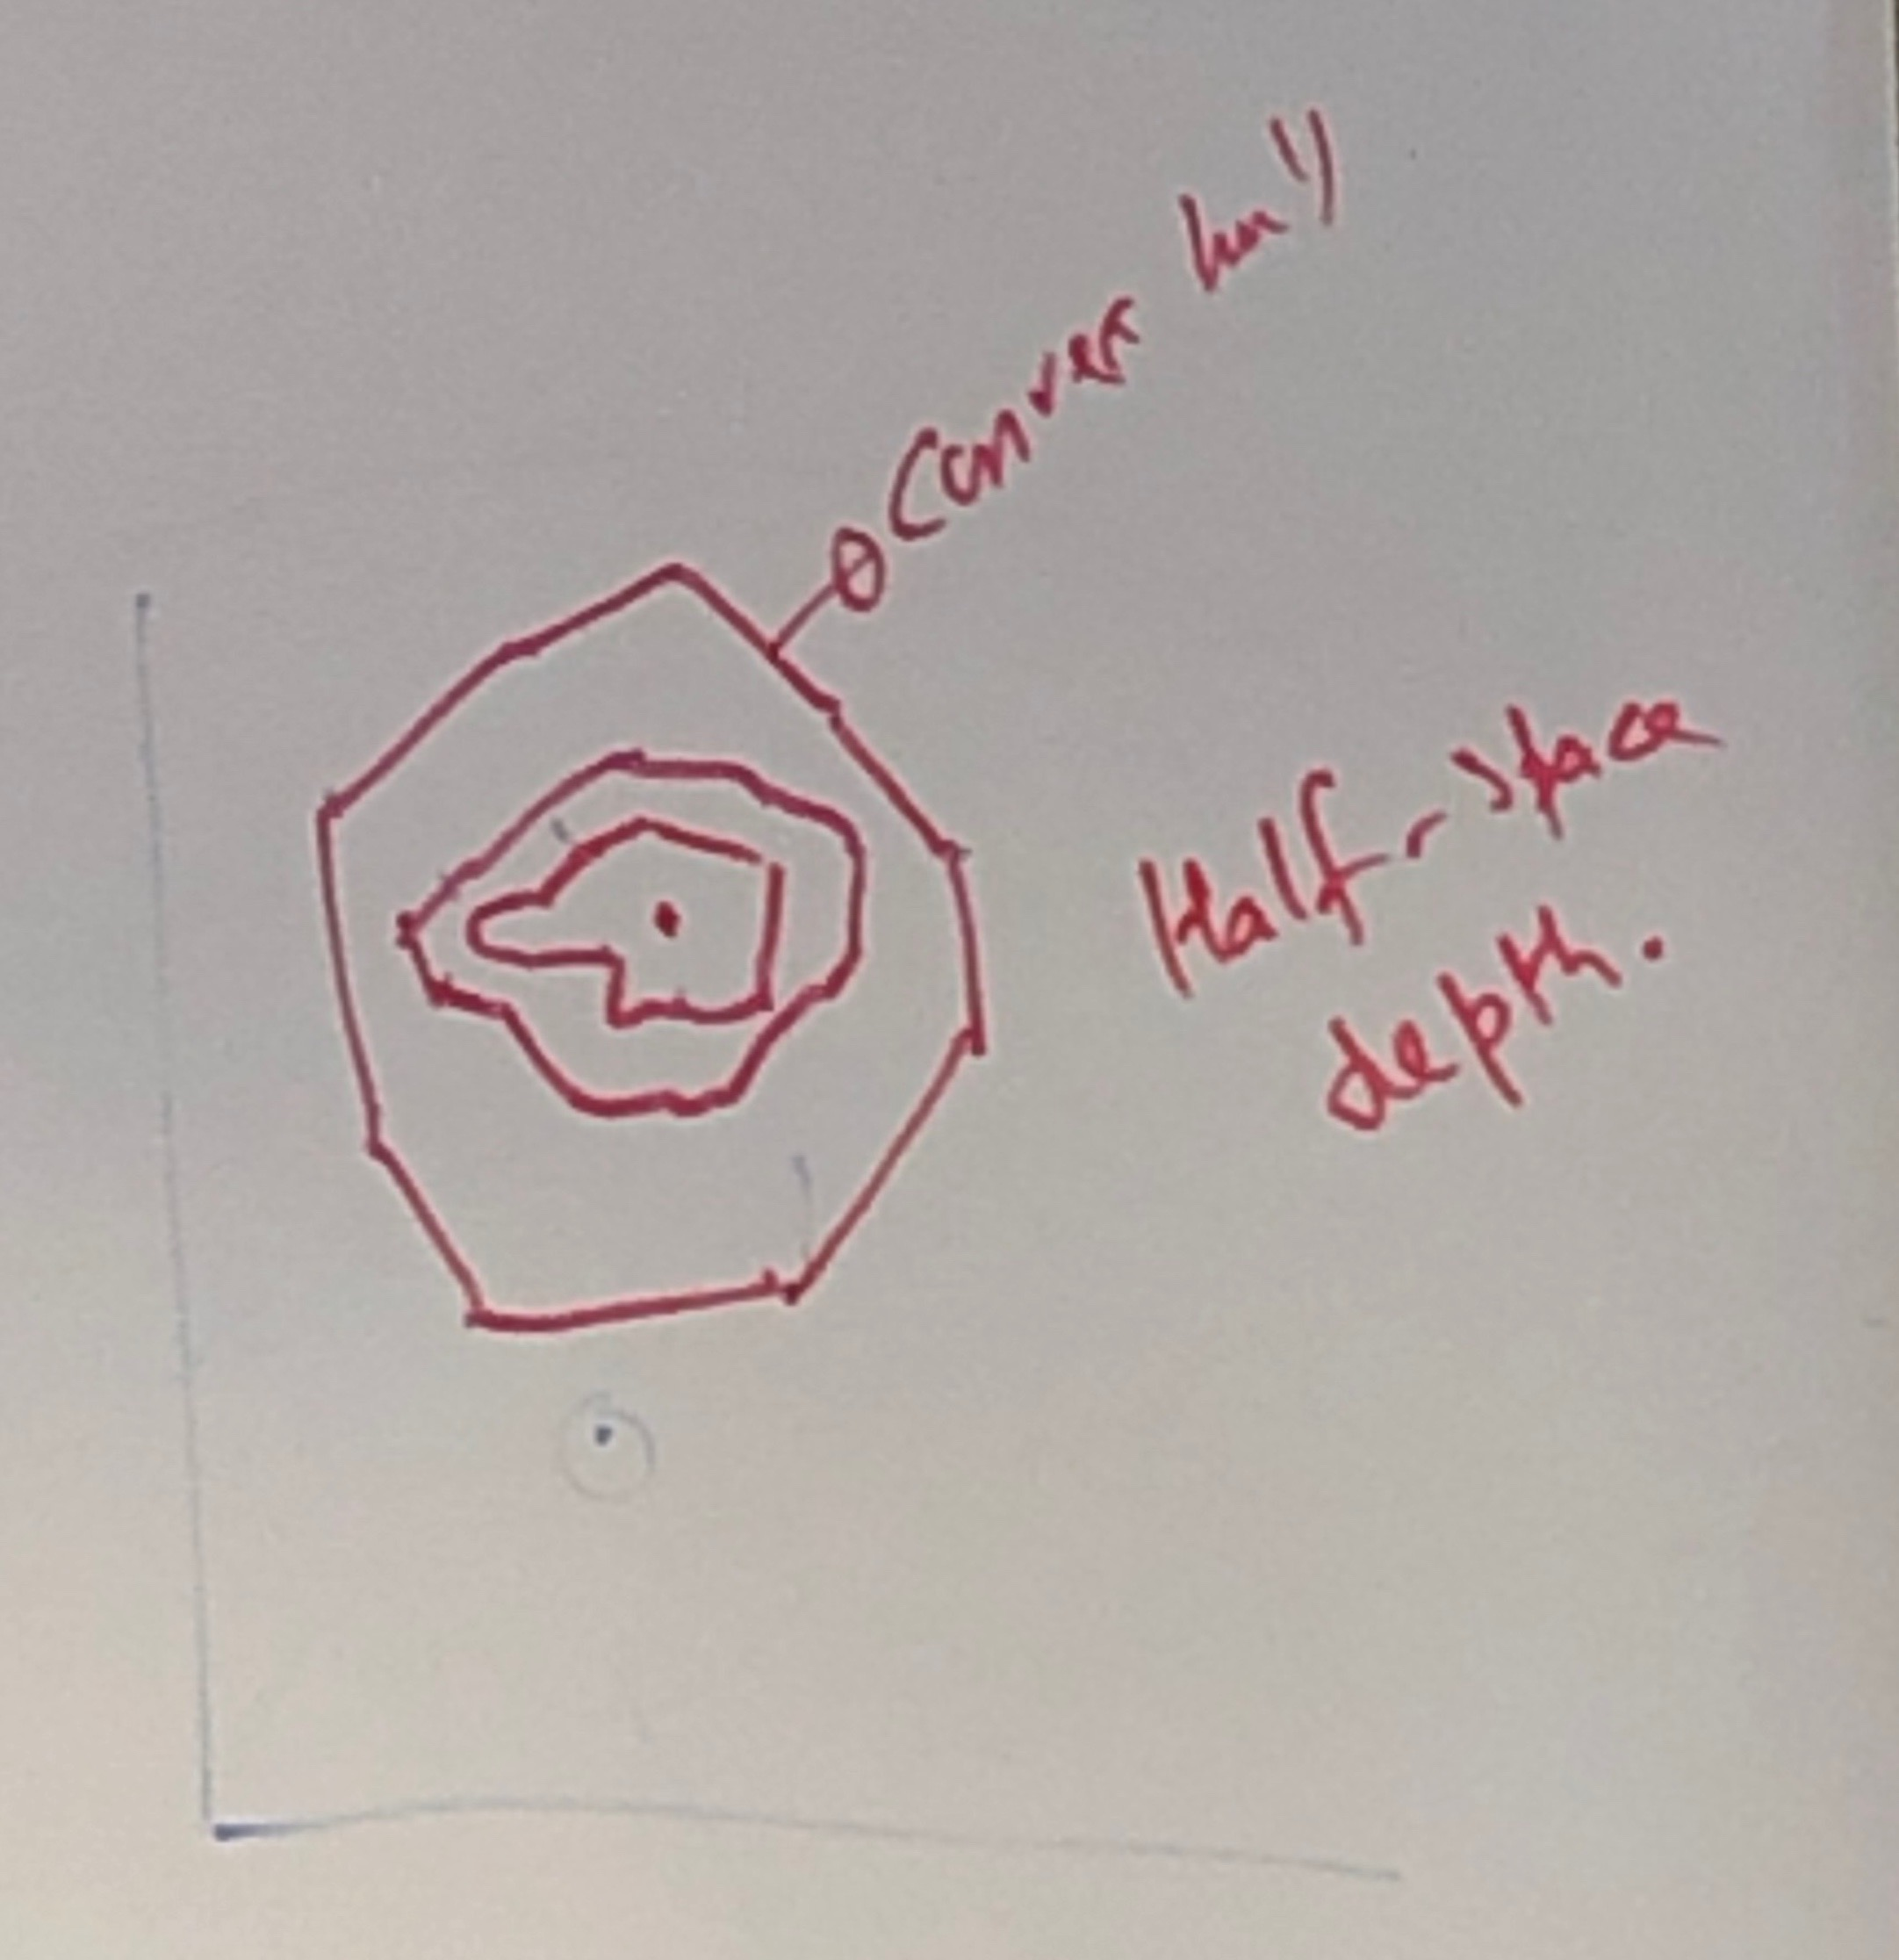
\includegraphics[scale=0.1]{linreg_half_space_depth}
\caption{Illustration of half-space depth method for detecting outliers.}
\label{linreg.fig.half.space.depth}
\end{center}
\end{figure}


\section{Transformed Linear Models}

\subsection{Transformations of response}

Consider the transformation

\[
t(y) = \begin{cases}
\frac{y^\lambda - 1}{\lambda} , & \lambda \neq 0 \\
\log(y) = \lim_{\lambda \to 0} \frac{y^\lambda - 1}{\lambda}, & \lambda = 0 
\end{cases}
\]

One example: \textbf{log linear model.}

\[
\log y_i = \beta_0 + \beta_1 x_i + \epsilon.
\]

Multiplicative model in the true response:

\[
y_i = \exp(\beta_0) \cdot \exp(x_1 \beta_1)  \cdot \exp(\epsilon_i)
\]

If you increase \(y_i\) by one unit, then \(y_i\) is multiplied by \(\exp(\beta_1)\). So in this case rather than talking about linear effects, you talk about percentage changes in the response: \((e^{\beta_1} - 1) \cdot 100 \%\).

Square root transformations work well in Poisson models---variance stabilizes. 

Consider

\[
t_\lambda = x'\beta + \epsilon.
\]

Then we have

\[
SSE = (t_\lambda - x_i' \hat{\beta}_{OLS})^T(t_\lambda - x_i' \hat{\beta}_{OLS}) 
\]

Try

\[
\frac{n}{2} \log \left(  \frac{SSE}{n} \right) + (\sum_{i=1}^n \log(y_i).
\]

for \(\lambda= -2, -2, -1/2, 0, 1/2, 1, 2\). We have \(2 L(\hat{\lambda}) - 2 L(\lambda_{true}) \sim \chi_1^2\). If 1 is inside the \(95\%\) confidence interval, don't transform; if 1 isn't, do. In a lot of cases, changing the response can be a pain for interpretability.

\subsection{Transforming predictor values}

Add polynomial terms:

\[
y_i = \beta_0 + \beta_1 x_i + \beta_2 x_i^2 + \ldots + \beta_d x_i^d + \epsilon.
\]

Want to maintain hierarchy in selecting variables (backward elimination). Advantages: nonlinear curvature. Global: all data have influence on every predicted point.

 
%%
%%
%%
%%
%%
%%
%%
%%
%%
%%%
%\bibliographystyle{abbrvnat}
%\bibliography{mybib2fin}
%\end{document}



